\section{Additional Evaluation}
\label{sec:eval-full}

This appendix reports the full GSM8K forest on Qwen3-14B (\S\ref{sec:eval-gpu}), details of the admission and probe experiments (\S\ref{sec:eval-grow}--\S\ref{sec:eval-wide}), a Qwen3-8B forest with an answer-marker decode stop (\S\ref{sec:eval-plus}), the multi-step sessions (\S\ref{sec:eval-mt}), cross-model results (\S\ref{sec:eval-multi}), and sensitivity to width, depth, and trace length (\S\ref{sec:eval-sens}).

\paragraph{Common setup.}
All runs use vLLM on four A100-SXM4 40GB GPUs with \texttt{bfloat16} weights, temperature $0$, and physically disaggregated prefill and decode instances connected by a KV connector.
Models are Qwen3-14B, Qwen3-8B, Qwen3-4B, Qwen2.5-Math-1.5B, Llama-3-8B-Instruct, Mistral-7B-Instruct, and DeepSeek-R1-Distill-Llama-8B (R1-8B).
Tree-of-Thoughts forests use $k{=}4$ and $D{=}512$ ($2048$ for contest problems) in batches of eight.
An answer is correct when its final number matches the reference; unless noted, accuracy is committed-answer accuracy.

\subsection{GSM8K Forest on Qwen3-14B}
\label{sec:eval-gpu}

The full GSM8K test set ($n{=}1319$) is run on Qwen3-14B at $\mathrm{tp}{=}2$ in $165$ batches of eight (\Cref{tab:gsm}).
This experiment isolates state management: no residual is rejected, so the copy-on-write tree is compared with recomputation and APC on the same committed path.

\begin{table}[t]
\centering
\caption{GSM8K test, Qwen3-14B, $\mathrm{tp}{=}2$, $n{=}1319$; medians over $165$ batches of eight.}
\label{tab:gsm}
\scriptsize
\setlength{\tabcolsep}{3.5pt}
\begin{tabular}{@{}lrrr@{}}
\toprule
 & recompute & APC & \cowonly \\
\midrule
Committed accuracy & $0.847$ & $0.844$ & $0.845$ \\
\rowcolor{tblalt}
Peak KV, median (tok) & $4136$ & $1430$ & \win{$1030$} \\
Peak KV, max (tok) & $4944$ & $1632$ & \win{$1232$} \\
\rowcolor{tblalt}
Peak / APC & $2.89\times$ & $1.00\times$ & \win{$0.72\times$} \\
Fan-out, median (ms) & $326$ & \win{$87$} & $140$ \\
\bottomrule
\end{tabular}
\end{table}

Median peak KV is $0.72\times$ APC and $0.25\times$ recomputation, and accuracy is within $0.3$ points of both.
Fan-out latency does not follow the same order: the copy-on-write fan-out takes $140$\,ms against $87$\,ms for APC, because fork and abort run on the expand path while an APC hit does not.
The same peak ordering ($0.58$--$0.80\times$ APC) holds on seven math datasets for Qwen3-14B, Qwen3-8B, and R1-8B at $\mathrm{tp}{=}2$ and $4$, and peak KV does not change with tensor-parallel width, consistent with \eqref{eq:mem}.

\begin{figure*}[t]
\centering
\resizebox{\textwidth}{!}{\begin{tikzpicture}[
  font=\scriptsize\sffamily,
  >=Latex,
]
\definecolor{Tr}{HTML}{7EB6D9}
\definecolor{Rs}{HTML}{F4A582}
\definecolor{Sp}{HTML}{66C2A5}
\definecolor{Cl}{HTML}{B3B3B3}

\node[font=\scriptsize\bfseries, anchor=west] at (0,5.55) {(a) Three systems, GSM8K $n{=}1319$ (one batch of eight)};

\begin{scope}[shift={(0,2.85)}]
  \foreach \y/\lab in {0/0, 2.1/2k, 4.2/4k} {
    \draw[black!12] (0,\y*0.476) -- (4.55,\y*0.476);
    \node[font=\tiny, text=black!50, anchor=east] at (-0.08,\y*0.476) {\lab};
  }
  \fill[Cl] (0.15,0) -- (1.00,1.48) -- (1.90,1.55) -- (4.40,1.55) -- (4.40,0) -- cycle;
  \fill[Rs] (1.00,1.48) -- (1.90,1.98) -- (4.40,1.98) -- (4.40,1.55) -- (1.90,1.55) -- cycle;
  \node[font=\tiny] at (2.80,0.78) {$79.2\%$};
  \node[font=\tiny, text=fsorange!80!black] at (2.80,1.76) {$20.8\%$};
  \foreach \x/\lab in {0.15/0, 1.90/40, 4.40/100} {
    \node[font=\tiny, text=black!50] at (\x,-0.22) {\lab};
  }
  \node[font=\tiny, anchor=south] at (2.25,2.10) {Recompute \quad peak $4136$};
\end{scope}

\begin{scope}[shift={(5.05,2.85)}]
  \foreach \y/\lab in {0/0, 0.75/0.8k, 1.50/1.5k} {
    \draw[black!12] (0,\y*1.333) -- (4.55,\y*1.333);
    \node[font=\tiny, text=black!50, anchor=east] at (-0.08,\y*1.333) {\lab};
  }
  \fill[Tr] (0.15,0) -- (1.00,1.25) -- (1.90,1.37) -- (4.40,1.37) -- (4.40,0) -- cycle;
  \fill[Rs] (1.00,1.25) -- (1.90,1.90) -- (4.40,1.90) -- (4.40,1.37) -- (1.90,1.37) -- cycle;
  \node[font=\tiny] at (2.80,0.68) {$68.4\%$};
  \node[font=\tiny, text=fsorange!80!black] at (2.80,1.64) {$31.6\%$};
  \foreach \x/\lab in {0.15/0, 1.90/40, 4.40/100} {
    \node[font=\tiny, text=black!50] at (\x,-0.22) {\lab};
  }
  \node[font=\tiny, anchor=south] at (2.25,2.10) {APC \quad peak $1430$};
\end{scope}

\begin{scope}[shift={(10.10,2.85)}]
  \foreach \y/\lab in {0/0, 0.55/0.6k, 1.10/1.1k} {
    \draw[black!12] (0,\y*1.818) -- (4.55,\y*1.818);
    \node[font=\tiny, text=black!50, anchor=east] at (-0.08,\y*1.818) {\lab};
  }
  \fill[Tr] (0.15,0) -- (1.00,1.55) -- (1.90,1.55) -- (2.55,1.55) -- (4.40,1.70) -- (4.40,0) -- cycle;
  \fill[Rs] (1.00,1.55) -- (1.90,1.95) -- (2.55,1.95) -- (2.55,1.55) -- cycle;
  \fill[Sp] (2.55,1.55) -- (4.40,1.87) -- (4.40,1.70) -- cycle;
  \node[font=\tiny] at (1.70,0.78) {$88.1\%$};
  \node[font=\tiny, text=fsorange!80!black] at (2.15,1.76) {$11.9\%$};
  \foreach \x/\lab in {0.15/0, 1.90/40, 4.40/100} {
    \node[font=\tiny, text=black!50] at (\x,-0.22) {\lab};
  }
  \node[font=\tiny, anchor=south] at (2.25,2.10) {\cowonly{} \quad peak $1030$};
\end{scope}

\node[font=\scriptsize\bfseries, anchor=west] at (0,2.35) {(b) Two workloads, $n{=}40$ (GSM8K vs.\ Game24)};

\begin{scope}[shift={(0,0)}]
  \foreach \y in {0,0.8,1.6} {
    \draw[black!12] (0,\y*0.95) -- (4.55,\y*0.95);
    \node[font=\tiny, text=black!50, anchor=east] at (-0.08,\y*0.95) {\y k};
  }
  \fill[Tr] (0.15,0) -- (1.20,0.68) -- (2.20,0.72) -- (4.40,0.72) -- (4.40,0) -- cycle;
  \fill[Rs] (0.15,0) -- (1.20,0.68) -- (2.20,1.34) -- (4.40,1.34) -- (4.40,0.72) -- (2.20,0.72) -- (1.20,0.68) -- cycle;
  \node[font=\tiny] at (3.10,0.36) {$54.0\%$};
  \node[font=\tiny, text=fsorange!80!black] at (3.10,1.02) {$46.0\%$};
  \foreach \x/\lab in {0.15/0, 2.20/50, 4.40/100} {
    \node[font=\tiny, text=black!50] at (\x,-0.20) {\lab};
  }
  \node[font=\tiny, anchor=south] at (2.25,1.68) {APC \quad $1512{+}1287$};
\end{scope}

\begin{scope}[shift={(5.05,0)}]
  \foreach \y in {0,0.8,1.6} {
    \draw[black!12] (0,\y*0.95) -- (4.55,\y*0.95);
  }
  \fill[Tr] (0.15,0) -- (1.20,0.50) -- (2.20,0.53) -- (4.40,0.53) -- (4.40,0) -- cycle;
  \fill[Sp] (1.20,0.50) -- (2.20,0.91) -- (4.40,0.91) -- (4.40,0.53) -- (2.20,0.53) -- cycle;
  \node[font=\tiny] at (3.10,0.26) {$58.4\%$};
  \node[font=\tiny, text=fsgreen!30!black] at (3.10,0.72) {$41.6\%$};
  \foreach \x/\lab in {0.15/0, 2.20/50, 4.40/100} {
    \node[font=\tiny, text=black!50] at (\x,-0.20) {\lab};
  }
  \node[font=\tiny, anchor=south] at (2.25,1.68) {\cowonly{} \quad $1112{+}791$};
\end{scope}

\begin{scope}[shift={(10.10,0)}]
  \foreach \y in {0,0.8,1.6} {
    \draw[black!12] (0,\y*0.95) -- (4.55,\y*0.95);
  }
  \fill[Tr] (0.15,0) -- (1.00,0.50) -- (1.80,0.53) -- (4.40,0.53) -- (4.40,0) -- cycle;
  \fill[Sp] (1.00,0.50) -- (1.80,0.82) -- (4.40,0.91) -- (4.40,0.53) -- (1.80,0.53) -- cycle;
  \node[font=\tiny] at (3.10,0.26) {$58.4\%$};
  \node[font=\tiny, text=fsgreen!30!black] at (3.10,0.72) {$41.6\%$};
  \foreach \x/\lab in {0.15/0, 2.20/50, 4.40/100} {
    \node[font=\tiny, text=black!50] at (\x,-0.20) {\lab};
  }
  \node[font=\tiny, anchor=south] at (2.25,1.68) {\sys{} \quad same $M$, less $W$};
\end{scope}

\fill[Cl] (0.15,-0.55) rectangle (0.38,-0.42);
\node[font=\tiny, anchor=west] at (0.44,-0.485) {trunk clones};
\fill[Tr] (2.35,-0.55) rectangle (2.58,-0.42);
\node[font=\tiny, anchor=west] at (2.64,-0.485) {shared trunk};
\fill[Rs] (4.85,-0.55) rectangle (5.08,-0.42);
\node[font=\tiny, anchor=west] at (5.14,-0.485) {residuals / Game24};
\fill[Sp] (8.05,-0.55) rectangle (8.28,-0.42);
\node[font=\tiny, anchor=west] at (8.34,-0.485) {committed spine};
\node[font=\tiny, text=black!55, anchor=west] at (11.15,-0.485)
  {Time is the expand$\rightarrow$abort$\rightarrow$decode phase. Peaks are measured.};
\end{tikzpicture}
}
\caption{\textbf{Stacked KV occupancy} over expand, abort, and decode.
(a)~One GSM8K batch of eight on Qwen3-14B (per-panel $y$-scale; peaks $4136$, $1430$, $1030$).
(b)~GSM8K (bottom) and Game of 24 (top), $n{=}40$, for APC, \cowonly, and \sys; \cowonly and \sys share $M$, and \sys computes fewer residual tokens.}
\label{fig:eval-stack}
\end{figure*}

\subsection{Probe Admission on MATH-500}
\label{sec:eval-grow}

The MATH-500 experiments use Qwen3-8B at $\mathrm{tp}{=}1$, the first $32$ problems of level $4$ or $5$, $D{=}1024$, and EOS ignored.
Half of the $k$ residuals are contest strategies; the other half alternate repetition loops and illegal text.
Coverage counts a problem when some branch that ran all $1024$ tokens is correct; the committed residual is index $0$.
Blanket rejection lowers coverage from $12/32$ to $6/32$ at $k{=}4$ and from $20/32$ to $13/32$ at $k{=}16$, whereas no loop residual yields a correct answer at any $k$, so rejecting loops does not reduce coverage.
At $k{=}16$ a $128$-token probe extends every illegal residual ($128/128$) and restores $20/32$ in $72.2$\,s instead of $104.1$\,s; probing the loops as well extends none of them and costs $74.4$\,s.
At $k{=}8$, $t_0{=}64$ reaches $16/32$ in $42.0$\,s, above the full fan-out ($15/32$ in $52.5$\,s); at $k{=}4$ no probe recovers $12/32$, and reject-only admission ($11/32$ in $23.0$\,s) is the closest setting.
\Cref{fig:eval-grow} plots \Cref{tab:grow}.

\begin{figure*}[t]
\centering
\resizebox{\textwidth}{!}{\begin{tikzpicture}[
  font=\scriptsize\sffamily,
  >=Latex,
  tick/.style={font=\tiny, text=black!55, inner sep=0pt},
  grid/.style={black!12, line width=0.25pt},
  ax/.style={black!55, line width=0.35pt},
  mk/.style={circle, inner sep=0pt, minimum size=2.6pt},
]
\definecolor{fullc}{HTML}{3D3D3D}
\definecolor{dropc}{HTML}{B00020}
\definecolor{skipc}{HTML}{5D6D7E}
\definecolor{g64c}{HTML}{D97B2F}
\definecolor{g128}{HTML}{0B6E4F}

\node[font=\tiny, anchor=west] at (0.15,3.55) {MATH-500, Qwen3-8B, $n{=}32$, $D{=}1024$, $\tau{=}0.45$};

\begin{scope}[shift={(0.85,0.15)}]
  \node[font=\tiny\bfseries, anchor=west] at (0,3.05) {(a) Any-finished};
  \foreach \y/\lab in {0.40/0, 1.55/10, 2.70/20} {
    \draw[grid] (0.4,\y) -- (6.15,\y);
    \node[tick, anchor=east] at (0.32,\y) {\lab};
  }
  \draw[ax] (0.4,0.40) -- (6.15,0.40);
  \draw[ax] (0.4,0.40) -- (0.4,2.85);
  \draw[fullc, line width=0.8pt] (1.6,1.780) -- (3.4,2.125) -- (5.2,2.700);
  \draw[dropc, dashed, line width=0.7pt] (1.6,1.090) -- (3.4,1.665) -- (5.2,1.895);
  \draw[skipc, densely dotted, line width=0.8pt] (1.6,1.665) -- (3.4,2.355) -- (5.2,2.240);
  \draw[g64c, line width=0.8pt] (1.6,1.320) -- (3.4,2.240) -- (5.2,2.470);
  \draw[g128, line width=0.95pt] (1.6,1.435) -- (3.4,1.895) -- (5.2,2.700);
  \foreach \x/\y in {1.6/1.780, 3.4/2.125, 5.2/2.700} {\fill[fullc] (\x,\y) circle (1.15pt);}
  \foreach \x/\y in {1.6/1.090, 3.4/1.665, 5.2/1.895} {\fill[dropc] (\x,\y) circle (1.15pt);}
  \foreach \x/\y in {1.6/1.665, 3.4/2.355, 5.2/2.240} {\fill[skipc] (\x,\y) circle (1.15pt);}
  \foreach \x/\y in {1.6/1.320, 3.4/2.240, 5.2/2.470} {\fill[g64c] (\x,\y) circle (1.15pt);}
  \foreach \x/\y in {1.6/1.435, 3.4/1.895, 5.2/2.700} {\draw[g128, line width=0.6pt, fill=white] (\x,\y) circle (1.7pt);}
  \node[font=\tiny, text=g128, anchor=south west] at (5.28,2.62) {$20$};
  \node[font=\tiny, text=dropc, anchor=north west] at (5.28,1.82) {$13$};
  \foreach \x/\lab in {1.6/4, 3.4/8, 5.2/16} {\node[tick] at (\x,0.18) {$k{=}\lab$};}
  \node[tick, rotate=90, anchor=south] at (-0.05,1.62) {of $32$};
\end{scope}

\begin{scope}[shift={(7.55,0.15)}]
  \node[font=\tiny\bfseries, anchor=west] at (0,3.05) {(b) End-to-end time};
  \foreach \y/\lab in {0.40/0, 1.446/50, 2.491/100} {
    \draw[grid] (0.4,\y) -- (6.15,\y);
    \node[tick, anchor=east] at (0.32,\y) {\lab};
  }
  \draw[ax] (0.4,0.40) -- (6.15,0.40);
  \draw[ax] (0.4,0.40) -- (0.4,2.85);
  \draw[fullc, line width=0.8pt] (1.6,0.929) -- (3.4,1.498) -- (5.2,2.577);
  \draw[dropc, dashed, line width=0.7pt] (1.6,0.799) -- (3.4,0.935) -- (5.2,1.489);
  \draw[skipc, densely dotted, line width=0.8pt] (1.6,0.881) -- (3.4,1.268) -- (5.2,1.893);
  \draw[g64c, line width=0.8pt] (1.6,0.902) -- (3.4,1.278) -- (5.2,1.916);
  \draw[g128, line width=0.95pt] (1.6,0.916) -- (3.4,1.305) -- (5.2,1.910);
  \foreach \x/\y in {1.6/0.929, 3.4/1.498, 5.2/2.577} {\fill[fullc] (\x,\y) circle (1.15pt);}
  \foreach \x/\y in {1.6/0.799, 3.4/0.935, 5.2/1.489} {\fill[dropc] (\x,\y) circle (1.15pt);}
  \foreach \x/\y in {1.6/0.881, 3.4/1.268, 5.2/1.893} {\fill[skipc] (\x,\y) circle (1.15pt);}
  \foreach \x/\y in {1.6/0.902, 3.4/1.278, 5.2/1.916} {\fill[g64c] (\x,\y) circle (1.15pt);}
  \foreach \x/\y in {1.6/0.916, 3.4/1.305, 5.2/1.910} {\draw[g128, line width=0.6pt, fill=white] (\x,\y) circle (1.7pt);}
  \node[font=\tiny, text=fullc, anchor=south] at (5.2,2.62) {$104.1$};
  \node[font=\tiny, text=g128, anchor=north] at (5.2,1.82) {$72.2$};
  \foreach \x/\lab in {1.6/4, 3.4/8, 5.2/16} {\node[tick] at (\x,0.18) {$k{=}\lab$};}
  \node[tick, rotate=90, anchor=south] at (-0.18,1.62) {seconds};
\end{scope}

\fill[fullc] (0.85,-0.42) rectangle (1.08,-0.26);
\node[font=\tiny, anchor=west] at (1.12,-0.34) {Full};
\draw[dropc, dashed, line width=0.7pt] (2.05,-0.34) -- (2.45,-0.34);
\node[font=\tiny, anchor=west] at (2.50,-0.34) {Drop $s{<}\tau$};
\draw[skipc, densely dotted, line width=0.8pt] (4.55,-0.34) -- (4.95,-0.34);
\node[font=\tiny, anchor=west] at (5.00,-0.34) {Skip loops};
\fill[g64c] (6.85,-0.42) rectangle (7.08,-0.26);
\node[font=\tiny, anchor=west] at (7.12,-0.34) {Grow $t_0{=}64$};
\draw[g128, line width=0.7pt, fill=white] (9.35,-0.34) circle (1.8pt);
\node[font=\tiny, anchor=west] at (9.55,-0.34) {Grow $t_0{=}128$};
\end{tikzpicture}
}
\caption{\textbf{Probe admission on MATH-500} (\Cref{tab:grow}).
Blanket rejection is fast but loses coverage; a $t_0{=}128$ probe returns to $20/32$ at $k{=}16$ in $72.2$\,s instead of $104.1$\,s.}
\label{fig:eval-grow}
\end{figure*}

\subsection{Admission on GSM8K}
\label{sec:eval-prefill}

The GSM8K admission experiments use the branching mix with $n{=}16$ and $D{=}512$ on Qwen3-8B at $\mathrm{tp}{=}1$.
Because the heuristic scores take three values on this mix (loop $0.02$, illegal $0.22$, live $\approx1$), any $\tau_{\mathrm{pre}}\in(0.02,0.22]$ yields the same admission set as $0.15$, and any $\tau_{\mathrm{pre}}\in(0.22,1)$ yields the same set as $0.45$; a denser threshold sweep therefore adds no information on this workload.
\Cref{fig:eval-admit} plots ESC across widths and the three hosts at $k{=}16$.
At $k{=}8$, reject-only admission keeps ESC at $16/16$ coverage ($10.84$ to $10.19$\,s) and raises Speculative Rejection and DPTS from $15/16$ to $16/16$.

\begin{figure*}[t]
\centering
\resizebox{\textwidth}{!}{\begin{tikzpicture}[
  font=\scriptsize\sffamily,
  >=Latex,
  tick/.style={font=\tiny, text=black!55, inner sep=0pt},
  grid/.style={black!12, line width=0.25pt},
  ax/.style={black!55, line width=0.35pt},
  bar/.style={draw=black!45, line width=0.2pt},
]
\definecolor{ESCc}{HTML}{C48A3A}
\definecolor{t15}{HTML}{D97B2F}
\definecolor{t45}{HTML}{4A2878}

\node[font=\tiny, anchor=west] at (0.05,3.35) {GSM8K, Qwen3-8B, $n{=}16$, $D{=}512$};

\begin{scope}[shift={(0.70,0.20)}]
  \node[font=\tiny\bfseries, anchor=west] at (0,2.95) {(a) End-to-end time};
  \foreach \y/\lab in {0.42/0, 1.20/6, 1.98/12, 2.76/18} {
    \draw[grid] (0.35,\y) -- (5.05,\y);
    \node[tick, anchor=east] at (0.28,\y) {\lab};
  }
  \draw[ax] (0.35,0.42) -- (5.05,0.42);
  \draw[ax] (0.35,0.42) -- (0.35,2.80);
  \draw[ESCc, line width=0.8pt] (1.35,1.545) -- (2.85,1.829) -- (4.35,2.637);
  \draw[t15, line width=0.8pt] (1.35,1.489) -- (2.85,1.745) -- (4.35,2.258);
  \draw[t45, line width=0.8pt] (1.35,1.446) -- (2.85,1.538) -- (4.35,1.841);
  \foreach \x/\y in {1.35/1.545, 2.85/1.829, 4.35/2.637} {\fill[ESCc] (\x,\y) circle (1.2pt);}
  \foreach \x/\y in {1.35/1.489, 2.85/1.745, 4.35/2.258} {\fill[t15] (\x,\y) circle (1.2pt);}
  \foreach \x/\y in {1.35/1.446, 2.85/1.538, 4.35/1.841} {\fill[t45] (\x,\y) circle (1.2pt);}
  \node[font=\tiny, text=t15, anchor=south] at (1.05,1.72) {$15/16$};
  \node[font=\tiny, text=t45, anchor=north] at (1.05,1.22) {$14/16$};
  \node[font=\tiny, text=t45, anchor=north] at (2.55,1.28) {$14/16$};
  \node[font=\tiny, text=black!55, anchor=south west] at (4.05,2.68) {$16/16$};
  \foreach \x/\lab in {1.35/4, 2.85/8, 4.35/16} {\node[tick] at (\x,0.22) {$k{=}\lab$};}
  \node[tick, rotate=90, anchor=south] at (-0.12,1.60) {seconds};
\end{scope}

\begin{scope}[shift={(6.15,0.20)}]
  \node[font=\tiny\bfseries, anchor=west] at (0,2.95) {(b) Computed prefill};
  \foreach \y/\lab in {0.42/0, 1.484/2.5k, 2.547/5k} {
    \draw[grid] (0.45,\y) -- (5.05,\y);
    \node[tick, anchor=east] at (0.38,\y) {\lab};
  }
  \draw[ax] (0.45,0.42) -- (5.05,0.42);
  \draw[ax] (0.45,0.42) -- (0.45,2.80);
  \draw[ESCc, line width=0.8pt] (1.35,0.982) -- (2.85,1.537) -- (4.35,2.551);
  \draw[t15, line width=0.8pt] (1.35,0.853) -- (2.85,1.279) -- (4.35,2.057);
  \draw[t45, line width=0.8pt] (1.35,0.731) -- (2.85,1.036) -- (4.35,1.598);
  \foreach \x/\y in {1.35/0.982, 2.85/1.537, 4.35/2.551} {\fill[ESCc] (\x,\y) circle (1.2pt);}
  \foreach \x/\y in {1.35/0.853, 2.85/1.279, 4.35/2.057} {\fill[t15] (\x,\y) circle (1.2pt);}
  \foreach \x/\y in {1.35/0.731, 2.85/1.036, 4.35/1.598} {\fill[t45] (\x,\y) circle (1.2pt);}
  \node[font=\tiny, text=ESCc, anchor=south] at (4.35,2.58) {$5008$};
  \node[font=\tiny, text=t15, anchor=west] at (4.42,1.98) {$3848$};
  \node[font=\tiny, text=t45, anchor=west] at (4.42,1.52) {$2768$};
  \foreach \x/\lab in {1.35/4, 2.85/8, 4.35/16} {\node[tick] at (\x,0.22) {$k{=}\lab$};}
  \node[tick, rotate=90, anchor=south] at (-0.08,1.60) {tokens};
\end{scope}

\begin{scope}[shift={(11.55,0.20)}]
  \node[font=\tiny\bfseries, anchor=west] at (0,2.95) {(c) $k{=}16$, three hosts};
  \foreach \y/\lab in {0.42/0, 1.20/6, 1.98/12, 2.76/18} {
    \draw[grid] (0.35,\y) -- (3.85,\y);
    \node[tick, anchor=east] at (0.28,\y) {\lab};
  }
  \draw[ax] (0.35,0.42) -- (3.85,0.42);
  \draw[ax] (0.35,0.42) -- (0.35,2.80);
  \fill[bar, ESCc] (0.70,0.42) rectangle (1.02,2.637);
  \fill[bar, t15] (1.08,0.42) rectangle (1.40,2.258);
  \fill[bar, ESCc] (1.85,0.42) rectangle (2.17,2.102);
  \fill[bar, t15] (2.23,0.42) rectangle (2.55,2.013);
  \fill[bar, ESCc] (3.00,0.42) rectangle (3.32,1.931);
  \fill[bar, t15] (3.38,0.42) rectangle (3.70,1.882);
  \node[font=\tiny, text=fsgain] at (1.24,2.72) {$-17\%$};
  \node[font=\tiny, text=fsgain] at (2.39,2.20) {$-5\%$};
  \node[font=\tiny, text=fsgain] at (3.54,2.02) {$-3\%$};
  \node[tick] at (1.05,0.22) {ESC};
  \node[tick] at (2.20,0.22) {SR};
  \node[tick] at (3.35,0.22) {DPTS};
  \node[tick, rotate=90, anchor=south] at (-0.12,1.60) {seconds};
\end{scope}

\fill[ESCc] (4.55,-0.38) rectangle (4.78,-0.22);
\node[font=\tiny, anchor=west] at (4.84,-0.30) {Host alone};
\fill[t15] (6.55,-0.38) rectangle (6.78,-0.22);
\node[font=\tiny, anchor=west] at (6.84,-0.30) {$\tau_{\mathrm{pre}}{=}0.15$};
\fill[t45] (9.15,-0.38) rectangle (9.38,-0.22);
\node[font=\tiny, anchor=west] at (9.44,-0.30) {$\tau_{\mathrm{pre}}{=}0.45$};
\node[font=\tiny, text=black!55, anchor=west] at (11.55,-0.30) {(c) gold $=$ host, orange $=$ $+\tau_{\mathrm{pre}}{=}0.15$};
\end{tikzpicture}
}
\caption{\textbf{Admission threshold on GSM8K} (\Cref{tab:prefill-bar,tab:main}).
(a)~ESC wall-clock across $k$, labeled with any-finished coverage.
(b)~Computed prefill: $-23\%$ at $\tau_{\mathrm{pre}}{=}0.15$ and $-45\%$ at $0.45$.
(c)~Reject-only admission in front of each host at $k{=}16$.}
\label{fig:eval-admit}
\end{figure*}

\subsection{Decode-Only, Prefill-Only, and Combined Pruning}
\label{sec:eval-ablate}

\Cref{tab:ablate-combine} (Appendix~\ref{sec:ablate-combine}) factorizes the $k{=}16$ results.
Decode-only pruning leaves $W$ at $5008$ tokens; prefill-only admission decodes every admitted residual to $D$; the combination retains the prefill reduction and adds the host's decode-time termination.
At $\tau_{\mathrm{pre}}{=}0.45$ the hosts terminate no additional residuals, because every residual they would terminate has already been rejected.

\subsection{Score-Based versus Winner-Only Admission}
\label{sec:eval-wide}

Admitting only index $0$ is a different policy from scoring every residual.
At $k{=}16$ and $\tau{=}0.45$, winner-only admission prefills $414$ tokens but lowers coverage to $11/16$ under ESC and $9/16$ under Speculative Rejection, while score-based admission of the eight residuals above $\tau$ prefills $2768$ tokens and retains $16/16$ (\Cref{tab:ablate-admit}).
Committed accuracy is similar for both policies ($9$--$11$ of $16$), so the difference lies in the coverage available to a better selector.

\paragraph{Capacity from measured peaks.}
For R1-8B on GSM8K ($n{=}16$, $k{=}4$), measured median peaks are $761$ tokens under APC and $561$ under the context tree.
With $32$ layers, $8$ KV heads of dimension $128$, and \texttt{bfloat16}, one token occupies $131072$ bytes, so an $8$\,GiB KV budget holds $65536$ tokens, i.e., $86$ APC trees or $116$ spines by \eqref{eq:slots} ($+35\%$).
This is an analytical capacity bound; we do not report SLO-constrained throughput, which would additionally depend on scheduling and batching.

\subsection{Qwen3-8B Forest with an Answer-Marker Stop}
\label{sec:eval-plus}

This experiment runs Qwen3-8B on GSM8K with $n{=}80$ and $D{=}512$ at $\mathrm{tp}{=}2$ and $4$; Game of 24 uses Tree-of-Thoughts with $k{=}4$, and HumanEval uses a ReAct wrap-and-recover loop with $k{=}2$.
The \sys runs additionally stop committed decode when the last non-empty line contains a finished answer, which reduces $D^{+}$ to about one third.
On this trace the scorer admits every issued residual, so the end-to-end ratio in \Cref{tab:plus} reflects the decode stop rather than admission.

\begin{table}[t]
\centering
\caption{Qwen3-8B forest, $n{=}80$, $D{=}512$.
\sys includes an answer-marker decode stop.
Peak KV does not depend on $\mathrm{tp}$; G24 and HE are the Game of 24 and HumanEval peaks.}
\label{tab:plus}
\scriptsize
\setlength{\tabcolsep}{2.4pt}
\begin{tabular}{@{}lrrrrrrr@{}}
\toprule
 & peak & $D^{+}$ & e2e (s) & acc. & e2e/APC & G24 & HE \\
\midrule
APC, $\mathrm{tp}{=}2$ & $1582$ & $40960$ & $36.0$ & $0.900$ & --- & $1289$ & $1970$ \\
\rowcolor{tblalt}
\sys, $\mathrm{tp}{=}2$ & \win{$1182$} & $13356$ & $28.2$ & $0.863$ & $0.78$ & \win{$793$} & \win{$1882$} \\
APC, $\mathrm{tp}{=}4$ & $1582$ & $40960$ & $22.7$ & $0.938$ & --- & $1289$ & $1970$ \\
\rowcolor{tblalt}
\sys, $\mathrm{tp}{=}4$ & \win{$1182$} & $12826$ & $16.9$ & $0.925$ & $0.75$ & \win{$793$} & \win{$1882$} \\
\bottomrule
\end{tabular}
\end{table}

Peak KV is $0.75\times$ APC on GSM8K, $0.62\times$ on Game of 24, and $0.96\times$ on HumanEval, where $k{=}2$ makes the residual a small fraction of the context.
Accuracy is $1$--$3$ points below APC ($0.863$ vs.\ $0.900$ at $\mathrm{tp}{=}2$; $0.925$ vs.\ $0.938$ at $\mathrm{tp}{=}4$), which we attribute to the decode stop truncating a few answers.

\subsection{Multi-Step Tree-of-Thoughts}
\label{sec:eval-mt}

Each problem is one session of $k{=}4$ candidates over three steps on Qwen3-4B and Qwen3-8B ($\mathrm{tp}{=}2$, $n{=}16$), issued as its own request.
Steps 1 and 2 decode a $32$-token step, abort the non-selected candidates, and promote the selected spine to the next trunk; step 3 decodes the final answer with $D{=}512$ (GSM8K) or $D{=}256$ (Game of 24).
On Game of 24 the steps propose an equation, continue on the remaining cards, and write the final expression; on GSM8K they set up the algebra, revise the previous step, and state the final number.
Admission runs before every fan-out, and the $32$-token step is decoded only for admitted residuals.
Per-phase timings are not comparable across systems, because the APC harness attributes step decoding to the expansion phase whereas ours attributes it to decode; \Cref{tab:mt} therefore reports end-to-end time only.

\begin{figure}[t]
\centering
\resizebox{\columnwidth}{!}{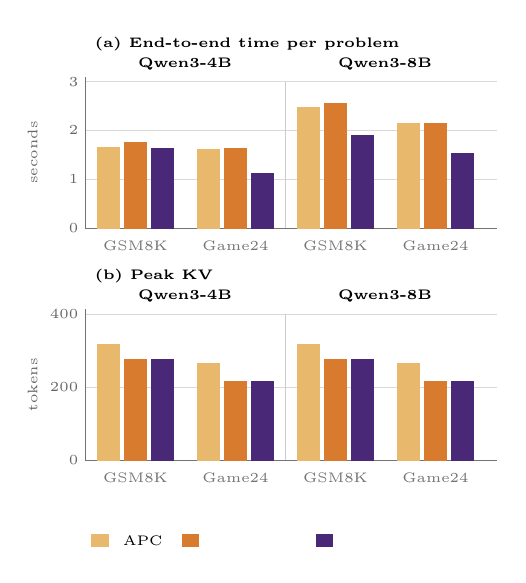
\begin{tikzpicture}[
  font=\scriptsize\sffamily,
  bar/.style={draw=black!55, line width=0.2pt},
  ax/.style={black!55, line width=0.35pt},
  grid/.style={black!15, line width=0.25pt},
  tick/.style={font=\tiny, text=black!60, inner sep=0pt},
  val/.style={font=\tiny, inner sep=0.2pt},
  wl/.style={font=\tiny, text=black!55, inner sep=0pt},
]
\definecolor{APC}{HTML}{E8B86D}
\definecolor{FS}{HTML}{D97B2F}
\definecolor{FSp}{HTML}{4A2878}

\begin{scope}[shift={(0,2.95)}]
  \node[font=\tiny\bfseries, anchor=west] at (0.62,2.72) {(a) End-to-end time per problem};
  \draw[grid] (0.62,0.38) -- (5.85,0.38);
  \draw[grid] (0.62,1.00) -- (5.85,1.00);
  \draw[grid] (0.62,1.62) -- (5.85,1.62);
  \draw[grid] (0.62,2.24) -- (5.85,2.24);
  \draw[ax] (0.62,0.38) -- (5.85,0.38);
  \draw[ax] (0.62,0.38) -- (0.62,2.30);
  \node[tick, anchor=east] at (0.54,0.38) {0};
  \node[tick, anchor=east] at (0.54,1.00) {1};
  \node[tick, anchor=east] at (0.54,1.62) {2};
  \node[tick, anchor=east] at (0.54,2.24) {3};
  \node[tick, rotate=90, anchor=south] at (0.02,1.34) {seconds};
  \node[font=\tiny\bfseries] at (1.89,2.46) {Qwen3-4B};
  \node[font=\tiny\bfseries] at (4.43,2.46) {Qwen3-8B};
  \draw[black!20] (3.16,0.38) -- (3.16,2.24);
  \fill[bar, APC] (0.78,0.38) rectangle (1.06,1.407);
  \fill[bar, FS]  (1.12,0.38) rectangle (1.40,1.474);
  \fill[bar, FSp] (1.46,0.38) rectangle (1.74,1.389);
  \node[wl] at (1.26,0.16) {GSM8K};
  \fill[bar, APC] (2.05,0.38) rectangle (2.33,1.379);
  \fill[bar, FS]  (2.39,0.38) rectangle (2.67,1.396);
  \fill[bar, FSp] (2.73,0.38) rectangle (3.01,1.079);
  \node[wl] at (2.53,0.16) {Game24};
  \fill[bar, APC] (3.32,0.38) rectangle (3.60,1.916);
  \fill[bar, FS]  (3.66,0.38) rectangle (3.94,1.968);
  \fill[bar, FSp] (4.00,0.38) rectangle (4.28,1.563);
  \node[wl] at (3.80,0.16) {GSM8K};
  \fill[bar, APC] (4.59,0.38) rectangle (4.87,1.713);
  \fill[bar, FS]  (4.93,0.38) rectangle (5.21,1.716);
  \fill[bar, FSp] (5.27,0.38) rectangle (5.55,1.324);
  \node[wl] at (5.07,0.16) {Game24};
\end{scope}

\begin{scope}[shift={(0,0)}]
  \node[font=\tiny\bfseries, anchor=west] at (0.62,2.72) {(b) Peak KV};
  \draw[grid] (0.62,0.38) -- (5.85,0.38);
  \draw[grid] (0.62,1.31) -- (5.85,1.31);
  \draw[grid] (0.62,2.24) -- (5.85,2.24);
  \draw[ax] (0.62,0.38) -- (5.85,0.38);
  \draw[ax] (0.62,0.38) -- (0.62,2.30);
  \node[tick, anchor=east] at (0.54,0.38) {0};
  \node[tick, anchor=east] at (0.54,1.31) {200};
  \node[tick, anchor=east] at (0.54,2.24) {400};
  \node[tick, rotate=90, anchor=south] at (0.02,1.34) {tokens};
  \node[font=\tiny\bfseries] at (1.89,2.46) {Qwen3-4B};
  \node[font=\tiny\bfseries] at (4.43,2.46) {Qwen3-8B};
  \draw[black!20] (3.16,0.38) -- (3.16,2.24);
  \fill[bar, APC] (0.78,0.38) rectangle (1.06,1.859);
  \fill[bar, FS]  (1.12,0.38) rectangle (1.40,1.659);
  \fill[bar, FSp] (1.46,0.38) rectangle (1.74,1.659);
  \node[wl] at (1.26,0.16) {GSM8K};
  \fill[bar, APC] (2.05,0.38) rectangle (2.33,1.612);
  \fill[bar, FS]  (2.39,0.38) rectangle (2.67,1.384);
  \fill[bar, FSp] (2.73,0.38) rectangle (3.01,1.384);
  \node[wl] at (2.53,0.16) {Game24};
  \fill[bar, APC] (3.32,0.38) rectangle (3.60,1.859);
  \fill[bar, FS]  (3.66,0.38) rectangle (3.94,1.659);
  \fill[bar, FSp] (4.00,0.38) rectangle (4.28,1.659);
  \node[wl] at (3.80,0.16) {GSM8K};
  \fill[bar, APC] (4.59,0.38) rectangle (4.87,1.612);
  \fill[bar, FS]  (4.93,0.38) rectangle (5.21,1.384);
  \fill[bar, FSp] (5.27,0.38) rectangle (5.55,1.384);
  \node[wl] at (5.07,0.16) {Game24};
\end{scope}

\fill[APC] (0.70,-0.72) rectangle (0.92,-0.56);
\node[font=\tiny, anchor=west] at (0.98,-0.64) {APC};
\fill[FS] (1.85,-0.72) rectangle (2.07,-0.56);
\node[font=\tiny, anchor=west] at (2.13,-0.64) {\cowonly};
\fill[FSp] (3.55,-0.72) rectangle (3.77,-0.56);
\node[font=\tiny, anchor=west] at (3.83,-0.64) {\sys};
\end{tikzpicture}
}
\caption{\textbf{Three-step Tree-of-Thoughts} ($n{=}16$, $\mathrm{tp}{=}2$).
(a)~End-to-end seconds per problem; \sys includes an answer-marker decode stop.
(b)~Peak KV of the live spine.}
\label{fig:eval-mt}
\end{figure}

\subsection{Cross-Model Results}
\label{sec:eval-multi}

The forest is repeated on six families ($n{=}40$, $D{=}512$, $\mathrm{tp}{=}2$ and $4$).
APC retains the shared trunk and all residuals, $M_{\mathrm{CoW}}=b(L+\sum_i\ell_i)$, while the context tree retains $M_{\mathrm{spine}}=b(L+\ell_\star)$; their ratio $(L+\ell_\star)/(L+\sum_i\ell_i)$ is independent of the model and of tensor-parallel width.
For similar residual lengths it reduces to $(L+\ell)/(L+k\ell)$, which decreases as $L/\ell$ decreases: $0.72$--$0.75$ on GSM8K with a long trunk and $0.57$--$0.61$ on Game of 24 with a short one (\Cref{fig:eval-multi}).
Relative to recomputation, which stores $M_{\mathrm{clone}}$, the spine is $0.25\times$.

\begin{figure*}[t]
\centering
\resizebox{\textwidth}{!}{\begin{tikzpicture}[
  font=\scriptsize\sffamily,
  bar/.style={draw=black!65, line width=0.22pt},
  >=Latex,
]
\definecolor{Rec}{HTML}{F8E6A0}
\definecolor{APC}{HTML}{E8B86D}
\definecolor{FS}{HTML}{D97B2F}
\definecolor{FSp}{HTML}{4A2878}

\fill[Rec] (4.10,7.48) rectangle (4.32,7.64);
\node[font=\tiny, anchor=west] at (4.36,7.56) {Recompute};
\fill[APC] (5.95,7.48) rectangle (6.17,7.64);
\node[font=\tiny, anchor=west] at (6.21,7.56) {APC};
\fill[FS] (7.15,7.48) rectangle (7.37,7.64);
\node[font=\tiny, anchor=west] at (7.41,7.56) {\cowonly};
\fill[FSp] (8.95,7.48) rectangle (9.17,7.64);
\node[font=\tiny, anchor=west] at (9.21,7.56) {\sys};

\begin{scope}[shift={(0.00,3.75)}]
  \node[font=\tiny\bfseries] at (2.20,3.41) {Qwen3-4B};
  \draw[black!12] (0.44,0.300) -- (4.18,0.300);
  \node[font=\tiny, text=black!45, anchor=east] at (0.38,0.300) {0};
  \draw[black!12] (0.44,1.119) -- (4.18,1.119);
  \node[font=\tiny, text=black!45, anchor=east] at (0.38,1.119) {1.5k};
  \draw[black!12] (0.44,1.939) -- (4.18,1.939);
  \node[font=\tiny, text=black!45, anchor=east] at (0.38,1.939) {3.0k};
  \draw[black!12] (0.44,2.758) -- (4.18,2.758);
  \node[font=\tiny, text=black!45, anchor=east] at (0.38,2.758) {4.5k};
  \draw[black!55] (0.44,0.30) -- (4.18,0.30);
  \draw[black!55] (0.44,0.30) -- (0.44,3.25);
  \fill[bar, Rec] (0.360,0.30) rectangle (0.660,2.739);
  \fill[bar, APC] (0.730,0.30) rectangle (1.030,1.126);
  \fill[bar, FS] (1.100,0.30) rectangle (1.400,0.907);
  \fill[bar, FSp] (1.470,0.30) rectangle (1.770,0.907);
  \node[font=\tiny, inner sep=0.2pt, fill=white, fill opacity=0.85, text opacity=1] at (0.510,2.879) {4464};
  \node[font=\tiny, inner sep=0.2pt, fill=white, fill opacity=0.85, text opacity=1] at (0.880,1.266) {1512};
  \node[font=\tiny, inner sep=0.2pt, fill=white, fill opacity=0.85, text opacity=1] at (1.435,1.047) {1112};
  \draw[black!75, line width=0.35pt] (0.880,1.126) -- (0.880,1.546);
  \draw[black!75, line width=0.35pt] (0.880,1.546) -- (1.250,1.546);
  \draw[black!75, line width=0.35pt] (1.250,1.546) -- (1.250,0.907);
  \node[font=\tiny\bfseries] at (1.065,1.696) {$0.74\times$};
  \node[font=\tiny, text=black!55] at (0.915,0.12) {GSM8K};
  \fill[bar, Rec] (2.280,0.30) rectangle (2.580,1.972);
  \fill[bar, APC] (2.650,0.30) rectangle (2.950,1.003);
  \fill[bar, FS] (3.020,0.30) rectangle (3.320,0.732);
  \fill[bar, FSp] (3.390,0.30) rectangle (3.690,0.732);
  \node[font=\tiny, inner sep=0.2pt, fill=white, fill opacity=0.85, text opacity=1] at (2.430,2.112) {3060};
  \node[font=\tiny, inner sep=0.2pt, fill=white, fill opacity=0.85, text opacity=1] at (2.800,1.143) {1287};
  \node[font=\tiny, inner sep=0.2pt, fill=white, fill opacity=0.85, text opacity=1] at (3.355,0.872) {791};
  \draw[black!75, line width=0.35pt] (2.800,1.003) -- (2.800,1.423);
  \draw[black!75, line width=0.35pt] (2.800,1.423) -- (3.170,1.423);
  \draw[black!75, line width=0.35pt] (3.170,1.423) -- (3.170,0.732);
  \node[font=\tiny\bfseries] at (2.985,1.573) {$0.61\times$};
  \node[font=\tiny, text=black!55] at (2.835,0.12) {Game24};
\end{scope}

\begin{scope}[shift={(5.25,3.75)}]
  \node[font=\tiny\bfseries] at (2.20,3.41) {Math-1.5B};
  \draw[black!12] (0.44,0.300) -- (4.18,0.300);
  \node[font=\tiny, text=black!45, anchor=east] at (0.38,0.300) {0};
  \draw[black!12] (0.44,1.119) -- (4.18,1.119);
  \node[font=\tiny, text=black!45, anchor=east] at (0.38,1.119) {1.5k};
  \draw[black!12] (0.44,1.939) -- (4.18,1.939);
  \node[font=\tiny, text=black!45, anchor=east] at (0.38,1.939) {3.0k};
  \draw[black!12] (0.44,2.758) -- (4.18,2.758);
  \node[font=\tiny, text=black!45, anchor=east] at (0.38,2.758) {4.5k};
  \draw[black!55] (0.44,0.30) -- (4.18,0.30);
  \draw[black!55] (0.44,0.30) -- (0.44,3.25);
  \fill[bar, Rec] (0.360,0.30) rectangle (0.660,2.739);
  \fill[bar, APC] (0.730,0.30) rectangle (1.030,1.126);
  \fill[bar, FS] (1.100,0.30) rectangle (1.400,0.907);
  \fill[bar, FSp] (1.470,0.30) rectangle (1.770,0.907);
  \node[font=\tiny, inner sep=0.2pt, fill=white, fill opacity=0.85, text opacity=1] at (0.510,2.879) {4464};
  \node[font=\tiny, inner sep=0.2pt, fill=white, fill opacity=0.85, text opacity=1] at (0.880,1.266) {1512};
  \node[font=\tiny, inner sep=0.2pt, fill=white, fill opacity=0.85, text opacity=1] at (1.435,1.047) {1112};
  \draw[black!75, line width=0.35pt] (0.880,1.126) -- (0.880,1.546);
  \draw[black!75, line width=0.35pt] (0.880,1.546) -- (1.250,1.546);
  \draw[black!75, line width=0.35pt] (1.250,1.546) -- (1.250,0.907);
  \node[font=\tiny\bfseries] at (1.065,1.696) {$0.74\times$};
  \node[font=\tiny, text=black!55] at (0.915,0.12) {GSM8K};
  \fill[bar, Rec] (2.280,0.30) rectangle (2.580,1.972);
  \fill[bar, APC] (2.650,0.30) rectangle (2.950,1.003);
  \fill[bar, FS] (3.020,0.30) rectangle (3.320,0.732);
  \fill[bar, FSp] (3.390,0.30) rectangle (3.690,0.732);
  \node[font=\tiny, inner sep=0.2pt, fill=white, fill opacity=0.85, text opacity=1] at (2.430,2.112) {3060};
  \node[font=\tiny, inner sep=0.2pt, fill=white, fill opacity=0.85, text opacity=1] at (2.800,1.143) {1287};
  \node[font=\tiny, inner sep=0.2pt, fill=white, fill opacity=0.85, text opacity=1] at (3.355,0.872) {791};
  \draw[black!75, line width=0.35pt] (2.800,1.003) -- (2.800,1.423);
  \draw[black!75, line width=0.35pt] (2.800,1.423) -- (3.170,1.423);
  \draw[black!75, line width=0.35pt] (3.170,1.423) -- (3.170,0.732);
  \node[font=\tiny\bfseries] at (2.985,1.573) {$0.61\times$};
  \node[font=\tiny, text=black!55] at (2.835,0.12) {Game24};
\end{scope}

\begin{scope}[shift={(10.50,3.75)}]
  \node[font=\tiny\bfseries] at (2.20,3.41) {Qwen3-14B};
  \draw[black!12] (0.44,0.300) -- (4.18,0.300);
  \node[font=\tiny, text=black!45, anchor=east] at (0.38,0.300) {0};
  \draw[black!12] (0.44,1.119) -- (4.18,1.119);
  \node[font=\tiny, text=black!45, anchor=east] at (0.38,1.119) {1.5k};
  \draw[black!12] (0.44,1.939) -- (4.18,1.939);
  \node[font=\tiny, text=black!45, anchor=east] at (0.38,1.939) {3.0k};
  \draw[black!12] (0.44,2.758) -- (4.18,2.758);
  \node[font=\tiny, text=black!45, anchor=east] at (0.38,2.758) {4.5k};
  \draw[black!55] (0.44,0.30) -- (4.18,0.30);
  \draw[black!55] (0.44,0.30) -- (0.44,3.25);
  \fill[bar, Rec] (0.360,0.30) rectangle (0.660,2.739);
  \fill[bar, APC] (0.730,0.30) rectangle (1.030,1.126);
  \fill[bar, FS] (1.100,0.30) rectangle (1.400,0.907);
  \fill[bar, FSp] (1.470,0.30) rectangle (1.770,0.907);
  \node[font=\tiny, inner sep=0.2pt, fill=white, fill opacity=0.85, text opacity=1] at (0.510,2.879) {4464};
  \node[font=\tiny, inner sep=0.2pt, fill=white, fill opacity=0.85, text opacity=1] at (0.880,1.266) {1512};
  \node[font=\tiny, inner sep=0.2pt, fill=white, fill opacity=0.85, text opacity=1] at (1.435,1.047) {1112};
  \draw[black!75, line width=0.35pt] (0.880,1.126) -- (0.880,1.546);
  \draw[black!75, line width=0.35pt] (0.880,1.546) -- (1.250,1.546);
  \draw[black!75, line width=0.35pt] (1.250,1.546) -- (1.250,0.907);
  \node[font=\tiny\bfseries] at (1.065,1.696) {$0.74\times$};
  \node[font=\tiny, text=black!55] at (0.915,0.12) {GSM8K};
  \fill[bar, Rec] (2.280,0.30) rectangle (2.580,1.972);
  \fill[bar, APC] (2.650,0.30) rectangle (2.950,1.003);
  \fill[bar, FS] (3.020,0.30) rectangle (3.320,0.732);
  \fill[bar, FSp] (3.390,0.30) rectangle (3.690,0.732);
  \node[font=\tiny, inner sep=0.2pt, fill=white, fill opacity=0.85, text opacity=1] at (2.430,2.112) {3060};
  \node[font=\tiny, inner sep=0.2pt, fill=white, fill opacity=0.85, text opacity=1] at (2.800,1.143) {1287};
  \node[font=\tiny, inner sep=0.2pt, fill=white, fill opacity=0.85, text opacity=1] at (3.355,0.872) {791};
  \draw[black!75, line width=0.35pt] (2.800,1.003) -- (2.800,1.423);
  \draw[black!75, line width=0.35pt] (2.800,1.423) -- (3.170,1.423);
  \draw[black!75, line width=0.35pt] (3.170,1.423) -- (3.170,0.732);
  \node[font=\tiny\bfseries] at (2.985,1.573) {$0.61\times$};
  \node[font=\tiny, text=black!55] at (2.835,0.12) {Game24};
\end{scope}

\begin{scope}[shift={(0.00,0.10)}]
  \node[font=\tiny\bfseries] at (2.20,3.41) {Llama-3-8B};
  \draw[black!12] (0.44,0.300) -- (4.18,0.300);
  \node[font=\tiny, text=black!45, anchor=east] at (0.38,0.300) {0};
  \draw[black!12] (0.44,1.119) -- (4.18,1.119);
  \node[font=\tiny, text=black!45, anchor=east] at (0.38,1.119) {1.5k};
  \draw[black!12] (0.44,1.939) -- (4.18,1.939);
  \node[font=\tiny, text=black!45, anchor=east] at (0.38,1.939) {3.0k};
  \draw[black!12] (0.44,2.758) -- (4.18,2.758);
  \node[font=\tiny, text=black!45, anchor=east] at (0.38,2.758) {4.5k};
  \draw[black!55] (0.44,0.30) -- (4.18,0.30);
  \draw[black!55] (0.44,0.30) -- (0.44,3.25);
  \fill[bar, Rec] (0.360,0.30) rectangle (0.660,2.732);
  \fill[bar, APC] (0.730,0.30) rectangle (1.030,1.124);
  \fill[bar, FS] (1.100,0.30) rectangle (1.400,0.906);
  \fill[bar, FSp] (1.470,0.30) rectangle (1.770,0.906);
  \node[font=\tiny, inner sep=0.2pt, fill=white, fill opacity=0.85, text opacity=1] at (0.510,2.872) {4452};
  \node[font=\tiny, inner sep=0.2pt, fill=white, fill opacity=0.85, text opacity=1] at (0.880,1.264) {1509};
  \node[font=\tiny, inner sep=0.2pt, fill=white, fill opacity=0.85, text opacity=1] at (1.435,1.046) {1109};
  \draw[black!75, line width=0.35pt] (0.880,1.124) -- (0.880,1.544);
  \draw[black!75, line width=0.35pt] (0.880,1.544) -- (1.250,1.544);
  \draw[black!75, line width=0.35pt] (1.250,1.544) -- (1.250,0.906);
  \node[font=\tiny\bfseries] at (1.065,1.694) {$0.73\times$};
  \node[font=\tiny, text=black!55] at (0.915,0.12) {GSM8K};
  \fill[bar, Rec] (2.280,0.30) rectangle (2.580,1.913);
  \fill[bar, APC] (2.650,0.30) rectangle (2.950,0.982);
  \fill[bar, FS] (3.020,0.30) rectangle (3.320,0.715);
  \fill[bar, FSp] (3.390,0.30) rectangle (3.690,0.715);
  \node[font=\tiny, inner sep=0.2pt, fill=white, fill opacity=0.85, text opacity=1] at (2.430,2.053) {2952};
  \node[font=\tiny, inner sep=0.2pt, fill=white, fill opacity=0.85, text opacity=1] at (2.800,1.122) {1248};
  \node[font=\tiny, inner sep=0.2pt, fill=white, fill opacity=0.85, text opacity=1] at (3.355,0.855) {760};
  \draw[black!75, line width=0.35pt] (2.800,0.982) -- (2.800,1.402);
  \draw[black!75, line width=0.35pt] (2.800,1.402) -- (3.170,1.402);
  \draw[black!75, line width=0.35pt] (3.170,1.402) -- (3.170,0.715);
  \node[font=\tiny\bfseries] at (2.985,1.552) {$0.61\times$};
  \node[font=\tiny, text=black!55] at (2.835,0.12) {Game24};
\end{scope}

\begin{scope}[shift={(5.25,0.10)}]
  \node[font=\tiny\bfseries] at (2.20,3.41) {Mistral-7B};
  \draw[black!12] (0.44,0.300) -- (4.18,0.300);
  \node[font=\tiny, text=black!45, anchor=east] at (0.38,0.300) {0};
  \draw[black!12] (0.44,1.119) -- (4.18,1.119);
  \node[font=\tiny, text=black!45, anchor=east] at (0.38,1.119) {1.5k};
  \draw[black!12] (0.44,1.939) -- (4.18,1.939);
  \node[font=\tiny, text=black!45, anchor=east] at (0.38,1.939) {3.0k};
  \draw[black!12] (0.44,2.758) -- (4.18,2.758);
  \node[font=\tiny, text=black!45, anchor=east] at (0.38,2.758) {4.5k};
  \draw[black!55] (0.44,0.30) -- (4.18,0.30);
  \draw[black!55] (0.44,0.30) -- (0.44,3.25);
  \fill[bar, Rec] (0.360,0.30) rectangle (0.660,2.850);
  \fill[bar, APC] (0.730,0.30) rectangle (1.030,1.157);
  \fill[bar, FS] (1.100,0.30) rectangle (1.400,0.939);
  \fill[bar, FSp] (1.470,0.30) rectangle (1.770,0.939);
  \node[font=\tiny, inner sep=0.2pt, fill=white, fill opacity=0.85, text opacity=1] at (0.510,2.990) {4668};
  \node[font=\tiny, inner sep=0.2pt, fill=white, fill opacity=0.85, text opacity=1] at (0.880,1.297) {1569};
  \node[font=\tiny, inner sep=0.2pt, fill=white, fill opacity=0.85, text opacity=1] at (1.435,1.079) {1169};
  \draw[black!75, line width=0.35pt] (0.880,1.157) -- (0.880,1.577);
  \draw[black!75, line width=0.35pt] (0.880,1.577) -- (1.250,1.577);
  \draw[black!75, line width=0.35pt] (1.250,1.577) -- (1.250,0.939);
  \node[font=\tiny\bfseries] at (1.065,1.727) {$0.75\times$};
  \node[font=\tiny, text=black!55] at (0.915,0.12) {GSM8K};
  \fill[bar, Rec] (2.280,0.30) rectangle (2.580,1.994);
  \fill[bar, APC] (2.650,0.30) rectangle (2.950,1.038);
  \fill[bar, FS] (3.020,0.30) rectangle (3.320,0.728);
  \fill[bar, FSp] (3.390,0.30) rectangle (3.690,0.728);
  \node[font=\tiny, inner sep=0.2pt, fill=white, fill opacity=0.85, text opacity=1] at (2.430,2.134) {3100};
  \node[font=\tiny, inner sep=0.2pt, fill=white, fill opacity=0.85, text opacity=1] at (2.800,1.178) {1351};
  \node[font=\tiny, inner sep=0.2pt, fill=white, fill opacity=0.85, text opacity=1] at (3.355,0.868) {783};
  \draw[black!75, line width=0.35pt] (2.800,1.038) -- (2.800,1.458);
  \draw[black!75, line width=0.35pt] (2.800,1.458) -- (3.170,1.458);
  \draw[black!75, line width=0.35pt] (3.170,1.458) -- (3.170,0.728);
  \node[font=\tiny\bfseries] at (2.985,1.608) {$0.58\times$};
  \node[font=\tiny, text=black!55] at (2.835,0.12) {Game24};
\end{scope}

\begin{scope}[shift={(10.50,0.10)}]
  \node[font=\tiny\bfseries] at (2.20,3.41) {DeepSeek-R1};
  \draw[black!12] (0.44,0.300) -- (4.18,0.300);
  \node[font=\tiny, text=black!45, anchor=east] at (0.38,0.300) {0};
  \draw[black!12] (0.44,1.119) -- (4.18,1.119);
  \node[font=\tiny, text=black!45, anchor=east] at (0.38,1.119) {1.5k};
  \draw[black!12] (0.44,1.939) -- (4.18,1.939);
  \node[font=\tiny, text=black!45, anchor=east] at (0.38,1.939) {3.0k};
  \draw[black!12] (0.44,2.758) -- (4.18,2.758);
  \node[font=\tiny, text=black!45, anchor=east] at (0.38,2.758) {4.5k};
  \draw[black!55] (0.44,0.30) -- (4.18,0.30);
  \draw[black!55] (0.44,0.30) -- (0.44,3.25);
  \fill[bar, Rec] (0.360,0.30) rectangle (0.660,2.505);
  \fill[bar, APC] (0.730,0.30) rectangle (1.030,1.068);
  \fill[bar, FS] (1.100,0.30) rectangle (1.400,0.849);
  \fill[bar, FSp] (1.470,0.30) rectangle (1.770,0.849);
  \node[font=\tiny, inner sep=0.2pt, fill=white, fill opacity=0.85, text opacity=1] at (0.510,2.645) {4036};
  \node[font=\tiny, inner sep=0.2pt, fill=white, fill opacity=0.85, text opacity=1] at (0.880,1.208) {1405};
  \node[font=\tiny, inner sep=0.2pt, fill=white, fill opacity=0.85, text opacity=1] at (1.435,0.989) {1005};
  \draw[black!75, line width=0.35pt] (0.880,1.068) -- (0.880,1.488);
  \draw[black!75, line width=0.35pt] (0.880,1.488) -- (1.250,1.488);
  \draw[black!75, line width=0.35pt] (1.250,1.488) -- (1.250,0.849);
  \node[font=\tiny\bfseries] at (1.065,1.638) {$0.72\times$};
  \node[font=\tiny, text=black!55] at (0.915,0.12) {GSM8K};
  \fill[bar, Rec] (2.280,0.30) rectangle (2.580,1.685);
  \fill[bar, APC] (2.650,0.30) rectangle (2.950,0.925);
  \fill[bar, FS] (3.020,0.30) rectangle (3.320,0.658);
  \fill[bar, FSp] (3.390,0.30) rectangle (3.690,0.658);
  \node[font=\tiny, inner sep=0.2pt, fill=white, fill opacity=0.85, text opacity=1] at (2.430,1.825) {2536};
  \node[font=\tiny, inner sep=0.2pt, fill=white, fill opacity=0.85, text opacity=1] at (2.800,1.065) {1144};
  \node[font=\tiny, inner sep=0.2pt, fill=white, fill opacity=0.85, text opacity=1] at (3.355,0.798) {656};
  \draw[black!75, line width=0.35pt] (2.800,0.925) -- (2.800,1.345);
  \draw[black!75, line width=0.35pt] (2.800,1.345) -- (3.170,1.345);
  \draw[black!75, line width=0.35pt] (3.170,1.345) -- (3.170,0.658);
  \node[font=\tiny\bfseries] at (2.985,1.495) {$0.57\times$};
  \node[font=\tiny, text=black!55] at (2.835,0.12) {Game24};
\end{scope}

\node[font=\tiny, text=black!55, rotate=90] at (-0.20,3.65) {Peak KV (tokens)};
\end{tikzpicture}

}
\caption{\textbf{Peak KV across six model families} ($n{=}40$, $\mathrm{tp}{=}2$).
Bars are recompute, APC, \cowonly, and \sys; \cowonly and \sys retain the same spine.
The annotated ratio is $M_{\mathrm{spine}}/M_{\mathrm{APC}}$.}
\label{fig:eval-multi}
\end{figure*}

\Cref{fig:eval-radar} repeats the comparison at $n{=}80$; \Cref{fig:eval-hist} shows per-item decode lengths.

\begin{figure}[t]
\centering
\resizebox{\columnwidth}{!}{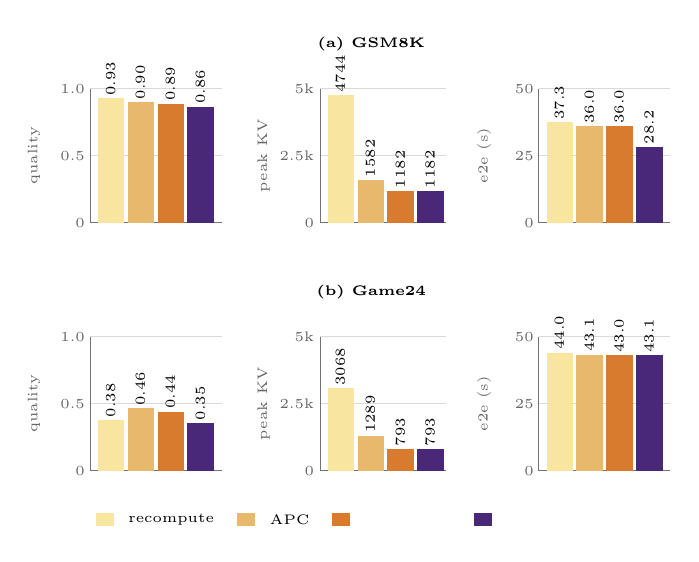
\begin{tikzpicture}[
  font=\scriptsize\sffamily,
  bar/.style={draw=black!55, line width=0.2pt},
  ax/.style={black!55, line width=0.35pt},
  grid/.style={black!15, line width=0.25pt},
  tick/.style={font=\tiny, text=black!60, inner sep=0pt},
  val/.style={font=\tiny, inner sep=0.3pt},
]
\definecolor{Rec}{HTML}{F8E6A0}
\definecolor{APC}{HTML}{E8B86D}
\definecolor{FS}{HTML}{D97B2F}
\definecolor{FSp}{HTML}{4A2878}

\begin{scope}[shift={(0,3.15)}]
  \node[font=\tiny\bfseries] at (4.05,2.55) {(a) GSM8K};
  \begin{scope}[shift={(0,0)}]
    \draw[grid] (0.48,0.28) -- (2.15,0.28) (0.48,1.13) -- (2.15,1.13) (0.48,1.98) -- (2.15,1.98);
    \draw[ax] (0.48,0.28) -- (2.15,0.28) (0.48,0.28) -- (0.48,1.98);
    \node[tick, anchor=east] at (0.42,0.28) {0};
    \node[tick, anchor=east] at (0.42,1.13) {0.5};
    \node[tick, anchor=east] at (0.42,1.98) {1.0};
    \node[tick, rotate=90, anchor=south] at (-0.15,1.13) {quality};
    \fill[bar, Rec] (0.58,0.28) rectangle (0.90,1.853);
    \fill[bar, APC] (0.96,0.28) rectangle (1.28,1.810);
    \fill[bar, FS]  (1.34,0.28) rectangle (1.66,1.788);
    \fill[bar, FSp] (1.72,0.28) rectangle (2.04,1.747);
    \node[val, rotate=90, anchor=west] at (0.74,1.87) {0.93};
    \node[val, rotate=90, anchor=west] at (1.12,1.83) {0.90};
    \node[val, rotate=90, anchor=west] at (1.50,1.81) {0.89};
    \node[val, rotate=90, anchor=west] at (1.88,1.77) {0.86};
  \end{scope}
  \begin{scope}[shift={(2.85,0)}]
    \draw[grid] (0.55,0.28) -- (2.15,0.28) (0.55,1.13) -- (2.15,1.13) (0.55,1.98) -- (2.15,1.98);
    \draw[ax] (0.55,0.28) -- (2.15,0.28) (0.55,0.28) -- (0.55,1.98);
    \node[tick, anchor=east] at (0.48,0.28) {0};
    \node[tick, anchor=east] at (0.48,1.13) {2.5k};
    \node[tick, anchor=east] at (0.48,1.98) {5k};
    \node[tick, rotate=90, anchor=south] at (-0.08,1.13) {peak KV};
    \fill[bar, Rec] (0.65,0.28) rectangle (0.97,1.893);
    \fill[bar, APC] (1.03,0.28) rectangle (1.35,0.818);
    \fill[bar, FS]  (1.41,0.28) rectangle (1.73,0.682);
    \fill[bar, FSp] (1.79,0.28) rectangle (2.11,0.682);
    \node[val, rotate=90, anchor=west] at (0.81,1.91) {4744};
    \node[val, rotate=90, anchor=west] at (1.19,0.84) {1582};
    \node[val, rotate=90, anchor=west] at (1.57,0.70) {1182};
    \node[val, rotate=90, anchor=west] at (1.95,0.70) {1182};
  \end{scope}
  \begin{scope}[shift={(5.70,0)}]
    \draw[grid] (0.48,0.28) -- (2.15,0.28) (0.48,1.13) -- (2.15,1.13) (0.48,1.98) -- (2.15,1.98);
    \draw[ax] (0.48,0.28) -- (2.15,0.28) (0.48,0.28) -- (0.48,1.98);
    \node[tick, anchor=east] at (0.42,0.28) {0};
    \node[tick, anchor=east] at (0.42,1.13) {25};
    \node[tick, anchor=east] at (0.42,1.98) {50};
    \node[tick, rotate=90, anchor=south] at (-0.12,1.13) {e2e (s)};
    \fill[bar, Rec] (0.58,0.28) rectangle (0.90,1.550);
    \fill[bar, APC] (0.96,0.28) rectangle (1.28,1.504);
    \fill[bar, FS]  (1.34,0.28) rectangle (1.66,1.505);
    \fill[bar, FSp] (1.72,0.28) rectangle (2.04,1.239);
    \node[val, rotate=90, anchor=west] at (0.74,1.57) {37.3};
    \node[val, rotate=90, anchor=west] at (1.12,1.52) {36.0};
    \node[val, rotate=90, anchor=west] at (1.50,1.52) {36.0};
    \node[val, rotate=90, anchor=west] at (1.88,1.26) {28.2};
  \end{scope}
\end{scope}

\begin{scope}[shift={(0,0)}]
  \node[font=\tiny\bfseries] at (4.05,2.55) {(b) Game24};
  \begin{scope}[shift={(0,0)}]
    \draw[grid] (0.48,0.28) -- (2.15,0.28) (0.48,1.13) -- (2.15,1.13) (0.48,1.98) -- (2.15,1.98);
    \draw[ax] (0.48,0.28) -- (2.15,0.28) (0.48,0.28) -- (0.48,1.98);
    \node[tick, anchor=east] at (0.42,0.28) {0};
    \node[tick, anchor=east] at (0.42,1.13) {0.5};
    \node[tick, anchor=east] at (0.42,1.98) {1.0};
    \node[tick, rotate=90, anchor=south] at (-0.15,1.13) {quality};
    \fill[bar, Rec] (0.58,0.28) rectangle (0.90,0.917);
    \fill[bar, APC] (0.96,0.28) rectangle (1.28,1.067);
    \fill[bar, FS]  (1.34,0.28) rectangle (1.66,1.025);
    \fill[bar, FSp] (1.72,0.28) rectangle (2.04,0.875);
    \node[val, rotate=90, anchor=west] at (0.74,0.94) {0.38};
    \node[val, rotate=90, anchor=west] at (1.12,1.09) {0.46};
    \node[val, rotate=90, anchor=west] at (1.50,1.05) {0.44};
    \node[val, rotate=90, anchor=west] at (1.88,0.90) {0.35};
  \end{scope}
  \begin{scope}[shift={(2.85,0)}]
    \draw[grid] (0.55,0.28) -- (2.15,0.28) (0.55,1.13) -- (2.15,1.13) (0.55,1.98) -- (2.15,1.98);
    \draw[ax] (0.55,0.28) -- (2.15,0.28) (0.55,0.28) -- (0.55,1.98);
    \node[tick, anchor=east] at (0.48,0.28) {0};
    \node[tick, anchor=east] at (0.48,1.13) {2.5k};
    \node[tick, anchor=east] at (0.48,1.98) {5k};
    \node[tick, rotate=90, anchor=south] at (-0.08,1.13) {peak KV};
    \fill[bar, Rec] (0.65,0.28) rectangle (0.97,1.323);
    \fill[bar, APC] (1.03,0.28) rectangle (1.35,0.718);
    \fill[bar, FS]  (1.41,0.28) rectangle (1.73,0.550);
    \fill[bar, FSp] (1.79,0.28) rectangle (2.11,0.550);
    \node[val, rotate=90, anchor=west] at (0.81,1.34) {3068};
    \node[val, rotate=90, anchor=west] at (1.19,0.74) {1289};
    \node[val, rotate=90, anchor=west] at (1.57,0.57) {793};
    \node[val, rotate=90, anchor=west] at (1.95,0.57) {793};
  \end{scope}
  \begin{scope}[shift={(5.70,0)}]
    \draw[grid] (0.48,0.28) -- (2.15,0.28) (0.48,1.13) -- (2.15,1.13) (0.48,1.98) -- (2.15,1.98);
    \draw[ax] (0.48,0.28) -- (2.15,0.28) (0.48,0.28) -- (0.48,1.98);
    \node[tick, anchor=east] at (0.42,0.28) {0};
    \node[tick, anchor=east] at (0.42,1.13) {25};
    \node[tick, anchor=east] at (0.42,1.98) {50};
    \node[tick, rotate=90, anchor=south] at (-0.12,1.13) {e2e (s)};
    \fill[bar, Rec] (0.58,0.28) rectangle (0.90,1.775);
    \fill[bar, APC] (0.96,0.28) rectangle (1.28,1.747);
    \fill[bar, FS]  (1.34,0.28) rectangle (1.66,1.741);
    \fill[bar, FSp] (1.72,0.28) rectangle (2.04,1.744);
    \node[val, rotate=90, anchor=west] at (0.74,1.80) {44.0};
    \node[val, rotate=90, anchor=west] at (1.12,1.77) {43.1};
    \node[val, rotate=90, anchor=west] at (1.50,1.76) {43.0};
    \node[val, rotate=90, anchor=west] at (1.88,1.76) {43.1};
  \end{scope}
\end{scope}

\fill[Rec] (0.55,-0.42) rectangle (0.78,-0.26);
\node[font=\tiny, anchor=west] at (0.84,-0.34) {recompute};
\fill[APC] (2.35,-0.42) rectangle (2.58,-0.26);
\node[font=\tiny, anchor=west] at (2.64,-0.34) {APC};
\fill[FS] (3.55,-0.42) rectangle (3.78,-0.26);
\node[font=\tiny, anchor=west] at (3.84,-0.34) {\cowonly};
\fill[FSp] (5.35,-0.42) rectangle (5.58,-0.26);
\node[font=\tiny, anchor=west] at (5.64,-0.34) {\sys};
\end{tikzpicture}
}
\caption{\textbf{Four systems on Qwen3-8B} ($n{=}80$, $\mathrm{tp}{=}2$, $D{=}512$).
Each panel has its own axis; for peak KV and end-to-end time shorter is better.
(a)~GSM8K. (b)~Game of 24.
\cowonly and \sys lower peak KV to $0.75\times$ (GSM8K) and $0.62\times$ (Game of 24) APC; the end-to-end reduction of \sys on GSM8K ($36.0$ to $28.2$\,s) is due to the answer-marker stop.}
\label{fig:eval-radar}
\end{figure}

\begin{figure*}[t]
\centering
\resizebox{\textwidth}{!}{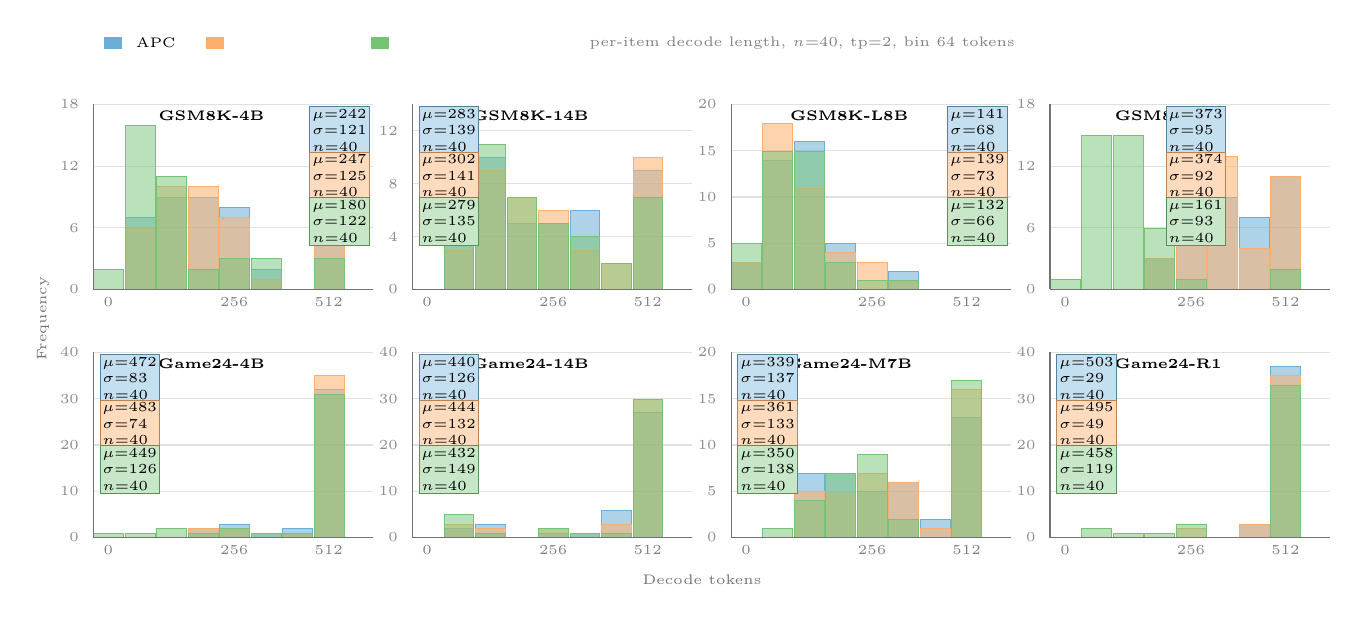
\begin{tikzpicture}[
  font=\scriptsize\sffamily,
  bar/.style={draw=black!50, line width=0.12pt},
]
\definecolor{APC}{HTML}{6BAED6}
\definecolor{FS}{HTML}{FDAE6B}
\definecolor{FSp}{HTML}{74C476}

\fill[APC] (0.55,6.62) rectangle (0.78,6.78);
\node[font=\tiny, anchor=west] at (0.84,6.70) {APC};
\fill[FS] (1.85,6.62) rectangle (2.08,6.78);
\node[font=\tiny, anchor=west] at (2.14,6.70) {\cowonly};
\fill[FSp] (3.95,6.62) rectangle (4.18,6.78);
\node[font=\tiny, anchor=west] at (4.24,6.70) {\sys};
\node[font=\tiny, text=black!50, anchor=west] at (6.6,6.70)
  {per-item decode length, $n{=}40$, $\mathrm{tp}{=}2$, bin $64$ tokens};

\begin{scope}[shift={(0.00,3.25)}]
  \node[font=\tiny\bfseries] at (1.92,2.53) {GSM8K-4B};
  \draw[black!12] (0.42,0.320) -- (3.97,0.320);
  \node[font=\tiny, text=black!45, anchor=east] at (0.36,0.320) {0};
  \draw[black!12] (0.42,1.103) -- (3.97,1.103);
  \node[font=\tiny, text=black!45, anchor=east] at (0.36,1.103) {6};
  \draw[black!12] (0.42,1.887) -- (3.97,1.887);
  \node[font=\tiny, text=black!45, anchor=east] at (0.36,1.887) {12};
  \draw[black!12] (0.42,2.670) -- (3.97,2.670);
  \node[font=\tiny, text=black!45, anchor=east] at (0.36,2.670) {18};
  \fill[bar, FSp, fill opacity=0.5] (0.420,0.32) rectangle (0.800,0.581);
  \fill[bar, APC, fill opacity=0.55] (0.820,0.32) rectangle (1.200,1.234);
  \fill[bar, FS, fill opacity=0.55] (0.820,0.32) rectangle (1.200,1.103);
  \fill[bar, FSp, fill opacity=0.5] (0.820,0.32) rectangle (1.200,2.409);
  \fill[bar, APC, fill opacity=0.55] (1.220,0.32) rectangle (1.600,1.495);
  \fill[bar, FS, fill opacity=0.55] (1.220,0.32) rectangle (1.600,1.626);
  \fill[bar, FSp, fill opacity=0.5] (1.220,0.32) rectangle (1.600,1.756);
  \fill[bar, APC, fill opacity=0.55] (1.620,0.32) rectangle (2.000,1.495);
  \fill[bar, FS, fill opacity=0.55] (1.620,0.32) rectangle (2.000,1.626);
  \fill[bar, FSp, fill opacity=0.5] (1.620,0.32) rectangle (2.000,0.581);
  \fill[bar, APC, fill opacity=0.55] (2.020,0.32) rectangle (2.400,1.364);
  \fill[bar, FS, fill opacity=0.55] (2.020,0.32) rectangle (2.400,1.234);
  \fill[bar, FSp, fill opacity=0.5] (2.020,0.32) rectangle (2.400,0.712);
  \fill[bar, APC, fill opacity=0.55] (2.420,0.32) rectangle (2.800,0.581);
  \fill[bar, FS, fill opacity=0.55] (2.420,0.32) rectangle (2.800,0.451);
  \fill[bar, FSp, fill opacity=0.5] (2.420,0.32) rectangle (2.800,0.712);
  \fill[bar, APC, fill opacity=0.55] (3.220,0.32) rectangle (3.600,0.973);
  \fill[bar, FS, fill opacity=0.55] (3.220,0.32) rectangle (3.600,1.103);
  \fill[bar, FSp, fill opacity=0.5] (3.220,0.32) rectangle (3.600,0.712);
  \draw[black!55] (0.42,0.32) -- (3.97,0.32);
  \draw[black!55] (0.42,0.32) -- (0.42,2.67);
  \node[font=\tiny, text=black!50] at (0.610,0.16) {0};
  \node[font=\tiny, text=black!50] at (2.210,0.16) {256};
  \node[font=\tiny, text=black!50] at (3.410,0.16) {512};
  \node[font=\tiny, inner sep=1.0pt, align=left, rectangle, fill=APC!40, draw=APC!75!black, line width=0.2pt, anchor=north east] at (3.93,2.65)
    {$\mu{=}242$\\$\sigma{=}121$\\$n{=}40$};
  \node[font=\tiny, inner sep=1.0pt, align=left, rectangle, fill=FS!45, draw=FS!75!black, line width=0.2pt, anchor=north east] at (3.93,2.07)
    {$\mu{=}247$\\$\sigma{=}125$\\$n{=}40$};
  \node[font=\tiny, inner sep=1.0pt, align=left, rectangle, fill=FSp!40, draw=FSp!75!black, line width=0.2pt, anchor=north east] at (3.93,1.49)
    {$\mu{=}180$\\$\sigma{=}122$\\$n{=}40$};
\end{scope}

\begin{scope}[shift={(4.05,3.25)}]
  \node[font=\tiny\bfseries] at (1.92,2.53) {GSM8K-14B};
  \draw[black!12] (0.42,0.320) -- (3.97,0.320);
  \node[font=\tiny, text=black!45, anchor=east] at (0.36,0.320) {0};
  \draw[black!12] (0.42,0.991) -- (3.97,0.991);
  \node[font=\tiny, text=black!45, anchor=east] at (0.36,0.991) {4};
  \draw[black!12] (0.42,1.663) -- (3.97,1.663);
  \node[font=\tiny, text=black!45, anchor=east] at (0.36,1.663) {8};
  \draw[black!12] (0.42,2.334) -- (3.97,2.334);
  \node[font=\tiny, text=black!45, anchor=east] at (0.36,2.334) {12};
  \fill[bar, APC, fill opacity=0.55] (0.820,0.32) rectangle (1.200,1.159);
  \fill[bar, FS, fill opacity=0.55] (0.820,0.32) rectangle (1.200,0.824);
  \fill[bar, FSp, fill opacity=0.5] (0.820,0.32) rectangle (1.200,0.991);
  \fill[bar, APC, fill opacity=0.55] (1.220,0.32) rectangle (1.600,1.999);
  \fill[bar, FS, fill opacity=0.55] (1.220,0.32) rectangle (1.600,1.831);
  \fill[bar, FSp, fill opacity=0.5] (1.220,0.32) rectangle (1.600,2.166);
  \fill[bar, APC, fill opacity=0.55] (1.620,0.32) rectangle (2.000,1.159);
  \fill[bar, FS, fill opacity=0.55] (1.620,0.32) rectangle (2.000,1.495);
  \fill[bar, FSp, fill opacity=0.5] (1.620,0.32) rectangle (2.000,1.495);
  \fill[bar, APC, fill opacity=0.55] (2.020,0.32) rectangle (2.400,1.159);
  \fill[bar, FS, fill opacity=0.55] (2.020,0.32) rectangle (2.400,1.327);
  \fill[bar, FSp, fill opacity=0.5] (2.020,0.32) rectangle (2.400,1.159);
  \fill[bar, APC, fill opacity=0.55] (2.420,0.32) rectangle (2.800,1.327);
  \fill[bar, FS, fill opacity=0.55] (2.420,0.32) rectangle (2.800,0.824);
  \fill[bar, FSp, fill opacity=0.5] (2.420,0.32) rectangle (2.800,0.991);
  \fill[bar, FS, fill opacity=0.55] (2.820,0.32) rectangle (3.200,0.656);
  \fill[bar, FSp, fill opacity=0.5] (2.820,0.32) rectangle (3.200,0.656);
  \fill[bar, APC, fill opacity=0.55] (3.220,0.32) rectangle (3.600,1.831);
  \fill[bar, FS, fill opacity=0.55] (3.220,0.32) rectangle (3.600,1.999);
  \fill[bar, FSp, fill opacity=0.5] (3.220,0.32) rectangle (3.600,1.495);
  \draw[black!55] (0.42,0.32) -- (3.97,0.32);
  \draw[black!55] (0.42,0.32) -- (0.42,2.67);
  \node[font=\tiny, text=black!50] at (0.610,0.16) {0};
  \node[font=\tiny, text=black!50] at (2.210,0.16) {256};
  \node[font=\tiny, text=black!50] at (3.410,0.16) {512};
  \node[font=\tiny, inner sep=1.0pt, align=left, rectangle, fill=APC!40, draw=APC!75!black, line width=0.2pt, anchor=north west] at (0.50,2.65)
    {$\mu{=}283$\\$\sigma{=}139$\\$n{=}40$};
  \node[font=\tiny, inner sep=1.0pt, align=left, rectangle, fill=FS!45, draw=FS!75!black, line width=0.2pt, anchor=north west] at (0.50,2.07)
    {$\mu{=}302$\\$\sigma{=}141$\\$n{=}40$};
  \node[font=\tiny, inner sep=1.0pt, align=left, rectangle, fill=FSp!40, draw=FSp!75!black, line width=0.2pt, anchor=north west] at (0.50,1.49)
    {$\mu{=}279$\\$\sigma{=}135$\\$n{=}40$};
\end{scope}

\begin{scope}[shift={(8.10,3.25)}]
  \node[font=\tiny\bfseries] at (1.92,2.53) {GSM8K-L8B};
  \draw[black!12] (0.42,0.320) -- (3.97,0.320);
  \node[font=\tiny, text=black!45, anchor=east] at (0.36,0.320) {0};
  \draw[black!12] (0.42,0.907) -- (3.97,0.907);
  \node[font=\tiny, text=black!45, anchor=east] at (0.36,0.907) {5};
  \draw[black!12] (0.42,1.495) -- (3.97,1.495);
  \node[font=\tiny, text=black!45, anchor=east] at (0.36,1.495) {10};
  \draw[black!12] (0.42,2.083) -- (3.97,2.083);
  \node[font=\tiny, text=black!45, anchor=east] at (0.36,2.083) {15};
  \draw[black!12] (0.42,2.670) -- (3.97,2.670);
  \node[font=\tiny, text=black!45, anchor=east] at (0.36,2.670) {20};
  \fill[bar, APC, fill opacity=0.55] (0.420,0.32) rectangle (0.800,0.672);
  \fill[bar, FS, fill opacity=0.55] (0.420,0.32) rectangle (0.800,0.672);
  \fill[bar, FSp, fill opacity=0.5] (0.420,0.32) rectangle (0.800,0.907);
  \fill[bar, APC, fill opacity=0.55] (0.820,0.32) rectangle (1.200,1.965);
  \fill[bar, FS, fill opacity=0.55] (0.820,0.32) rectangle (1.200,2.435);
  \fill[bar, FSp, fill opacity=0.5] (0.820,0.32) rectangle (1.200,2.083);
  \fill[bar, APC, fill opacity=0.55] (1.220,0.32) rectangle (1.600,2.200);
  \fill[bar, FS, fill opacity=0.55] (1.220,0.32) rectangle (1.600,1.613);
  \fill[bar, FSp, fill opacity=0.5] (1.220,0.32) rectangle (1.600,2.083);
  \fill[bar, APC, fill opacity=0.55] (1.620,0.32) rectangle (2.000,0.907);
  \fill[bar, FS, fill opacity=0.55] (1.620,0.32) rectangle (2.000,0.790);
  \fill[bar, FSp, fill opacity=0.5] (1.620,0.32) rectangle (2.000,0.672);
  \fill[bar, FS, fill opacity=0.55] (2.020,0.32) rectangle (2.400,0.672);
  \fill[bar, FSp, fill opacity=0.5] (2.020,0.32) rectangle (2.400,0.438);
  \fill[bar, APC, fill opacity=0.55] (2.420,0.32) rectangle (2.800,0.555);
  \fill[bar, FS, fill opacity=0.55] (2.420,0.32) rectangle (2.800,0.438);
  \fill[bar, FSp, fill opacity=0.5] (2.420,0.32) rectangle (2.800,0.438);
  \draw[black!55] (0.42,0.32) -- (3.97,0.32);
  \draw[black!55] (0.42,0.32) -- (0.42,2.67);
  \node[font=\tiny, text=black!50] at (0.610,0.16) {0};
  \node[font=\tiny, text=black!50] at (2.210,0.16) {256};
  \node[font=\tiny, text=black!50] at (3.410,0.16) {512};
  \node[font=\tiny, inner sep=1.0pt, align=left, rectangle, fill=APC!40, draw=APC!75!black, line width=0.2pt, anchor=north east] at (3.93,2.65)
    {$\mu{=}141$\\$\sigma{=}68$\\$n{=}40$};
  \node[font=\tiny, inner sep=1.0pt, align=left, rectangle, fill=FS!45, draw=FS!75!black, line width=0.2pt, anchor=north east] at (3.93,2.07)
    {$\mu{=}139$\\$\sigma{=}73$\\$n{=}40$};
  \node[font=\tiny, inner sep=1.0pt, align=left, rectangle, fill=FSp!40, draw=FSp!75!black, line width=0.2pt, anchor=north east] at (3.93,1.49)
    {$\mu{=}132$\\$\sigma{=}66$\\$n{=}40$};
\end{scope}

\begin{scope}[shift={(12.15,3.25)}]
  \node[font=\tiny\bfseries] at (1.92,2.53) {GSM8K-R1};
  \draw[black!12] (0.42,0.320) -- (3.97,0.320);
  \node[font=\tiny, text=black!45, anchor=east] at (0.36,0.320) {0};
  \draw[black!12] (0.42,1.103) -- (3.97,1.103);
  \node[font=\tiny, text=black!45, anchor=east] at (0.36,1.103) {6};
  \draw[black!12] (0.42,1.887) -- (3.97,1.887);
  \node[font=\tiny, text=black!45, anchor=east] at (0.36,1.887) {12};
  \draw[black!12] (0.42,2.670) -- (3.97,2.670);
  \node[font=\tiny, text=black!45, anchor=east] at (0.36,2.670) {18};
  \fill[bar, FSp, fill opacity=0.5] (0.420,0.32) rectangle (0.800,0.451);
  \fill[bar, FSp, fill opacity=0.5] (0.820,0.32) rectangle (1.200,2.278);
  \fill[bar, FSp, fill opacity=0.5] (1.220,0.32) rectangle (1.600,2.278);
  \fill[bar, APC, fill opacity=0.55] (1.620,0.32) rectangle (2.000,0.712);
  \fill[bar, FS, fill opacity=0.55] (1.620,0.32) rectangle (2.000,0.712);
  \fill[bar, FSp, fill opacity=0.5] (1.620,0.32) rectangle (2.000,1.103);
  \fill[bar, APC, fill opacity=0.55] (2.020,0.32) rectangle (2.400,1.626);
  \fill[bar, FS, fill opacity=0.55] (2.020,0.32) rectangle (2.400,1.495);
  \fill[bar, FSp, fill opacity=0.5] (2.020,0.32) rectangle (2.400,0.451);
  \fill[bar, APC, fill opacity=0.55] (2.420,0.32) rectangle (2.800,1.495);
  \fill[bar, FS, fill opacity=0.55] (2.420,0.32) rectangle (2.800,2.017);
  \fill[bar, APC, fill opacity=0.55] (2.820,0.32) rectangle (3.200,1.234);
  \fill[bar, FS, fill opacity=0.55] (2.820,0.32) rectangle (3.200,0.842);
  \fill[bar, APC, fill opacity=0.55] (3.220,0.32) rectangle (3.600,1.756);
  \fill[bar, FS, fill opacity=0.55] (3.220,0.32) rectangle (3.600,1.756);
  \fill[bar, FSp, fill opacity=0.5] (3.220,0.32) rectangle (3.600,0.581);
  \draw[black!55] (0.42,0.32) -- (3.97,0.32);
  \draw[black!55] (0.42,0.32) -- (0.42,2.67);
  \node[font=\tiny, text=black!50] at (0.610,0.16) {0};
  \node[font=\tiny, text=black!50] at (2.210,0.16) {256};
  \node[font=\tiny, text=black!50] at (3.410,0.16) {512};
  \node[font=\tiny, inner sep=1.0pt, align=left, rectangle, fill=APC!40, draw=APC!75!black, line width=0.2pt, anchor=north] at (2.27,2.65)
    {$\mu{=}373$\\$\sigma{=}95$\\$n{=}40$};
  \node[font=\tiny, inner sep=1.0pt, align=left, rectangle, fill=FS!45, draw=FS!75!black, line width=0.2pt, anchor=north] at (2.27,2.07)
    {$\mu{=}374$\\$\sigma{=}92$\\$n{=}40$};
  \node[font=\tiny, inner sep=1.0pt, align=left, rectangle, fill=FSp!40, draw=FSp!75!black, line width=0.2pt, anchor=north] at (2.27,1.49)
    {$\mu{=}161$\\$\sigma{=}93$\\$n{=}40$};
\end{scope}

\begin{scope}[shift={(0.00,0.10)}]
  \node[font=\tiny\bfseries] at (1.92,2.53) {Game24-4B};
  \draw[black!12] (0.42,0.320) -- (3.97,0.320);
  \node[font=\tiny, text=black!45, anchor=east] at (0.36,0.320) {0};
  \draw[black!12] (0.42,0.907) -- (3.97,0.907);
  \node[font=\tiny, text=black!45, anchor=east] at (0.36,0.907) {10};
  \draw[black!12] (0.42,1.495) -- (3.97,1.495);
  \node[font=\tiny, text=black!45, anchor=east] at (0.36,1.495) {20};
  \draw[black!12] (0.42,2.083) -- (3.97,2.083);
  \node[font=\tiny, text=black!45, anchor=east] at (0.36,2.083) {30};
  \draw[black!12] (0.42,2.670) -- (3.97,2.670);
  \node[font=\tiny, text=black!45, anchor=east] at (0.36,2.670) {40};
  \fill[bar, FSp, fill opacity=0.5] (0.420,0.32) rectangle (0.800,0.379);
  \fill[bar, FSp, fill opacity=0.5] (0.820,0.32) rectangle (1.200,0.379);
  \fill[bar, FSp, fill opacity=0.5] (1.220,0.32) rectangle (1.600,0.438);
  \fill[bar, APC, fill opacity=0.55] (1.620,0.32) rectangle (2.000,0.438);
  \fill[bar, FS, fill opacity=0.55] (1.620,0.32) rectangle (2.000,0.438);
  \fill[bar, FSp, fill opacity=0.5] (1.620,0.32) rectangle (2.000,0.379);
  \fill[bar, APC, fill opacity=0.55] (2.020,0.32) rectangle (2.400,0.496);
  \fill[bar, FS, fill opacity=0.55] (2.020,0.32) rectangle (2.400,0.438);
  \fill[bar, FSp, fill opacity=0.5] (2.020,0.32) rectangle (2.400,0.438);
  \fill[bar, APC, fill opacity=0.55] (2.420,0.32) rectangle (2.800,0.379);
  \fill[bar, FSp, fill opacity=0.5] (2.420,0.32) rectangle (2.800,0.379);
  \fill[bar, APC, fill opacity=0.55] (2.820,0.32) rectangle (3.200,0.438);
  \fill[bar, FS, fill opacity=0.55] (2.820,0.32) rectangle (3.200,0.379);
  \fill[bar, FSp, fill opacity=0.5] (2.820,0.32) rectangle (3.200,0.379);
  \fill[bar, APC, fill opacity=0.55] (3.220,0.32) rectangle (3.600,2.200);
  \fill[bar, FS, fill opacity=0.55] (3.220,0.32) rectangle (3.600,2.376);
  \fill[bar, FSp, fill opacity=0.5] (3.220,0.32) rectangle (3.600,2.141);
  \draw[black!55] (0.42,0.32) -- (3.97,0.32);
  \draw[black!55] (0.42,0.32) -- (0.42,2.67);
  \node[font=\tiny, text=black!50] at (0.610,0.16) {0};
  \node[font=\tiny, text=black!50] at (2.210,0.16) {256};
  \node[font=\tiny, text=black!50] at (3.410,0.16) {512};
  \node[font=\tiny, inner sep=1.0pt, align=left, rectangle, fill=APC!40, draw=APC!75!black, line width=0.2pt, anchor=north west] at (0.50,2.65)
    {$\mu{=}472$\\$\sigma{=}83$\\$n{=}40$};
  \node[font=\tiny, inner sep=1.0pt, align=left, rectangle, fill=FS!45, draw=FS!75!black, line width=0.2pt, anchor=north west] at (0.50,2.07)
    {$\mu{=}483$\\$\sigma{=}74$\\$n{=}40$};
  \node[font=\tiny, inner sep=1.0pt, align=left, rectangle, fill=FSp!40, draw=FSp!75!black, line width=0.2pt, anchor=north west] at (0.50,1.49)
    {$\mu{=}449$\\$\sigma{=}126$\\$n{=}40$};
\end{scope}

\begin{scope}[shift={(4.05,0.10)}]
  \node[font=\tiny\bfseries] at (1.92,2.53) {Game24-14B};
  \draw[black!12] (0.42,0.320) -- (3.97,0.320);
  \node[font=\tiny, text=black!45, anchor=east] at (0.36,0.320) {0};
  \draw[black!12] (0.42,0.907) -- (3.97,0.907);
  \node[font=\tiny, text=black!45, anchor=east] at (0.36,0.907) {10};
  \draw[black!12] (0.42,1.495) -- (3.97,1.495);
  \node[font=\tiny, text=black!45, anchor=east] at (0.36,1.495) {20};
  \draw[black!12] (0.42,2.083) -- (3.97,2.083);
  \node[font=\tiny, text=black!45, anchor=east] at (0.36,2.083) {30};
  \draw[black!12] (0.42,2.670) -- (3.97,2.670);
  \node[font=\tiny, text=black!45, anchor=east] at (0.36,2.670) {40};
  \fill[bar, APC, fill opacity=0.55] (0.820,0.32) rectangle (1.200,0.438);
  \fill[bar, FS, fill opacity=0.55] (0.820,0.32) rectangle (1.200,0.496);
  \fill[bar, FSp, fill opacity=0.5] (0.820,0.32) rectangle (1.200,0.614);
  \fill[bar, APC, fill opacity=0.55] (1.220,0.32) rectangle (1.600,0.496);
  \fill[bar, FS, fill opacity=0.55] (1.220,0.32) rectangle (1.600,0.438);
  \fill[bar, FSp, fill opacity=0.5] (1.220,0.32) rectangle (1.600,0.379);
  \fill[bar, APC, fill opacity=0.55] (2.020,0.32) rectangle (2.400,0.379);
  \fill[bar, FS, fill opacity=0.55] (2.020,0.32) rectangle (2.400,0.438);
  \fill[bar, FSp, fill opacity=0.5] (2.020,0.32) rectangle (2.400,0.438);
  \fill[bar, APC, fill opacity=0.55] (2.420,0.32) rectangle (2.800,0.379);
  \fill[bar, FSp, fill opacity=0.5] (2.420,0.32) rectangle (2.800,0.379);
  \fill[bar, APC, fill opacity=0.55] (2.820,0.32) rectangle (3.200,0.672);
  \fill[bar, FS, fill opacity=0.55] (2.820,0.32) rectangle (3.200,0.496);
  \fill[bar, FSp, fill opacity=0.5] (2.820,0.32) rectangle (3.200,0.379);
  \fill[bar, APC, fill opacity=0.55] (3.220,0.32) rectangle (3.600,1.906);
  \fill[bar, FS, fill opacity=0.55] (3.220,0.32) rectangle (3.600,2.083);
  \fill[bar, FSp, fill opacity=0.5] (3.220,0.32) rectangle (3.600,2.083);
  \draw[black!55] (0.42,0.32) -- (3.97,0.32);
  \draw[black!55] (0.42,0.32) -- (0.42,2.67);
  \node[font=\tiny, text=black!50] at (0.610,0.16) {0};
  \node[font=\tiny, text=black!50] at (2.210,0.16) {256};
  \node[font=\tiny, text=black!50] at (3.410,0.16) {512};
  \node[font=\tiny, inner sep=1.0pt, align=left, rectangle, fill=APC!40, draw=APC!75!black, line width=0.2pt, anchor=north west] at (0.50,2.65)
    {$\mu{=}440$\\$\sigma{=}126$\\$n{=}40$};
  \node[font=\tiny, inner sep=1.0pt, align=left, rectangle, fill=FS!45, draw=FS!75!black, line width=0.2pt, anchor=north west] at (0.50,2.07)
    {$\mu{=}444$\\$\sigma{=}132$\\$n{=}40$};
  \node[font=\tiny, inner sep=1.0pt, align=left, rectangle, fill=FSp!40, draw=FSp!75!black, line width=0.2pt, anchor=north west] at (0.50,1.49)
    {$\mu{=}432$\\$\sigma{=}149$\\$n{=}40$};
\end{scope}

\begin{scope}[shift={(8.10,0.10)}]
  \node[font=\tiny\bfseries] at (1.92,2.53) {Game24-M7B};
  \draw[black!12] (0.42,0.320) -- (3.97,0.320);
  \node[font=\tiny, text=black!45, anchor=east] at (0.36,0.320) {0};
  \draw[black!12] (0.42,0.907) -- (3.97,0.907);
  \node[font=\tiny, text=black!45, anchor=east] at (0.36,0.907) {5};
  \draw[black!12] (0.42,1.495) -- (3.97,1.495);
  \node[font=\tiny, text=black!45, anchor=east] at (0.36,1.495) {10};
  \draw[black!12] (0.42,2.083) -- (3.97,2.083);
  \node[font=\tiny, text=black!45, anchor=east] at (0.36,2.083) {15};
  \draw[black!12] (0.42,2.670) -- (3.97,2.670);
  \node[font=\tiny, text=black!45, anchor=east] at (0.36,2.670) {20};
  \fill[bar, FSp, fill opacity=0.5] (0.820,0.32) rectangle (1.200,0.438);
  \fill[bar, APC, fill opacity=0.55] (1.220,0.32) rectangle (1.600,1.143);
  \fill[bar, FS, fill opacity=0.55] (1.220,0.32) rectangle (1.600,0.907);
  \fill[bar, FSp, fill opacity=0.5] (1.220,0.32) rectangle (1.600,0.790);
  \fill[bar, APC, fill opacity=0.55] (1.620,0.32) rectangle (2.000,1.143);
  \fill[bar, FS, fill opacity=0.55] (1.620,0.32) rectangle (2.000,0.907);
  \fill[bar, FSp, fill opacity=0.5] (1.620,0.32) rectangle (2.000,1.143);
  \fill[bar, APC, fill opacity=0.55] (2.020,0.32) rectangle (2.400,0.907);
  \fill[bar, FS, fill opacity=0.55] (2.020,0.32) rectangle (2.400,1.143);
  \fill[bar, FSp, fill opacity=0.5] (2.020,0.32) rectangle (2.400,1.378);
  \fill[bar, APC, fill opacity=0.55] (2.420,0.32) rectangle (2.800,1.025);
  \fill[bar, FS, fill opacity=0.55] (2.420,0.32) rectangle (2.800,1.025);
  \fill[bar, FSp, fill opacity=0.5] (2.420,0.32) rectangle (2.800,0.555);
  \fill[bar, APC, fill opacity=0.55] (2.820,0.32) rectangle (3.200,0.555);
  \fill[bar, FS, fill opacity=0.55] (2.820,0.32) rectangle (3.200,0.438);
  \fill[bar, APC, fill opacity=0.55] (3.220,0.32) rectangle (3.600,1.848);
  \fill[bar, FS, fill opacity=0.55] (3.220,0.32) rectangle (3.600,2.200);
  \fill[bar, FSp, fill opacity=0.5] (3.220,0.32) rectangle (3.600,2.317);
  \draw[black!55] (0.42,0.32) -- (3.97,0.32);
  \draw[black!55] (0.42,0.32) -- (0.42,2.67);
  \node[font=\tiny, text=black!50] at (0.610,0.16) {0};
  \node[font=\tiny, text=black!50] at (2.210,0.16) {256};
  \node[font=\tiny, text=black!50] at (3.410,0.16) {512};
  \node[font=\tiny, inner sep=1.0pt, align=left, rectangle, fill=APC!40, draw=APC!75!black, line width=0.2pt, anchor=north west] at (0.50,2.65)
    {$\mu{=}339$\\$\sigma{=}137$\\$n{=}40$};
  \node[font=\tiny, inner sep=1.0pt, align=left, rectangle, fill=FS!45, draw=FS!75!black, line width=0.2pt, anchor=north west] at (0.50,2.07)
    {$\mu{=}361$\\$\sigma{=}133$\\$n{=}40$};
  \node[font=\tiny, inner sep=1.0pt, align=left, rectangle, fill=FSp!40, draw=FSp!75!black, line width=0.2pt, anchor=north west] at (0.50,1.49)
    {$\mu{=}350$\\$\sigma{=}138$\\$n{=}40$};
\end{scope}

\begin{scope}[shift={(12.15,0.10)}]
  \node[font=\tiny\bfseries] at (1.92,2.53) {Game24-R1};
  \draw[black!12] (0.42,0.320) -- (3.97,0.320);
  \node[font=\tiny, text=black!45, anchor=east] at (0.36,0.320) {0};
  \draw[black!12] (0.42,0.907) -- (3.97,0.907);
  \node[font=\tiny, text=black!45, anchor=east] at (0.36,0.907) {10};
  \draw[black!12] (0.42,1.495) -- (3.97,1.495);
  \node[font=\tiny, text=black!45, anchor=east] at (0.36,1.495) {20};
  \draw[black!12] (0.42,2.083) -- (3.97,2.083);
  \node[font=\tiny, text=black!45, anchor=east] at (0.36,2.083) {30};
  \draw[black!12] (0.42,2.670) -- (3.97,2.670);
  \node[font=\tiny, text=black!45, anchor=east] at (0.36,2.670) {40};
  \fill[bar, FSp, fill opacity=0.5] (0.820,0.32) rectangle (1.200,0.438);
  \fill[bar, FSp, fill opacity=0.5] (1.220,0.32) rectangle (1.600,0.379);
  \fill[bar, FSp, fill opacity=0.5] (1.620,0.32) rectangle (2.000,0.379);
  \fill[bar, FS, fill opacity=0.55] (2.020,0.32) rectangle (2.400,0.438);
  \fill[bar, FSp, fill opacity=0.5] (2.020,0.32) rectangle (2.400,0.496);
  \fill[bar, APC, fill opacity=0.55] (2.820,0.32) rectangle (3.200,0.496);
  \fill[bar, FS, fill opacity=0.55] (2.820,0.32) rectangle (3.200,0.496);
  \fill[bar, APC, fill opacity=0.55] (3.220,0.32) rectangle (3.600,2.494);
  \fill[bar, FS, fill opacity=0.55] (3.220,0.32) rectangle (3.600,2.376);
  \fill[bar, FSp, fill opacity=0.5] (3.220,0.32) rectangle (3.600,2.259);
  \draw[black!55] (0.42,0.32) -- (3.97,0.32);
  \draw[black!55] (0.42,0.32) -- (0.42,2.67);
  \node[font=\tiny, text=black!50] at (0.610,0.16) {0};
  \node[font=\tiny, text=black!50] at (2.210,0.16) {256};
  \node[font=\tiny, text=black!50] at (3.410,0.16) {512};
  \node[font=\tiny, inner sep=1.0pt, align=left, rectangle, fill=APC!40, draw=APC!75!black, line width=0.2pt, anchor=north west] at (0.50,2.65)
    {$\mu{=}503$\\$\sigma{=}29$\\$n{=}40$};
  \node[font=\tiny, inner sep=1.0pt, align=left, rectangle, fill=FS!45, draw=FS!75!black, line width=0.2pt, anchor=north west] at (0.50,2.07)
    {$\mu{=}495$\\$\sigma{=}49$\\$n{=}40$};
  \node[font=\tiny, inner sep=1.0pt, align=left, rectangle, fill=FSp!40, draw=FSp!75!black, line width=0.2pt, anchor=north west] at (0.50,1.49)
    {$\mu{=}458$\\$\sigma{=}119$\\$n{=}40$};
\end{scope}

\node[font=\tiny, text=black!55, rotate=90] at (-0.22,3.20) {Frequency};
\node[font=\tiny, text=black!55] at (8.15,-0.12) {Decode tokens};
\end{tikzpicture}

}
\caption{\textbf{Per-item decode-length histograms} ($n{=}40$, $\mathrm{tp}{=}2$, $D{=}512$, bin width $64$).
GSM8K (top) and Game of 24 (bottom) overlay APC, \cowonly, and \sys; boxes report $\mu$, $\sigma$, and $n$.
Llama-3-8B on Game of 24 is omitted because every output has length $1$; Mistral-7B is shown instead.}
\label{fig:eval-hist}
\end{figure*}

\Cref{tab:r1stop} isolates the answer-marker stop on three further models ($n{=}32$).
The stop reduces $D^{+}$ by $23$--$69\%$ and leaves the spine peak unchanged, but its effect on accuracy is model-dependent: $+2$ problems on R1-8B, $-1$ on Llama-3-8B, and $-5$ on Mistral-7B ($0.344$ to $0.188$), where the model emits intermediate answer markers before finishing.
The stop is therefore not a safe default and is not part of the admission results in \S\ref{sec:eval}.

\begin{table}[t]
\centering
\caption{Spine peak and an optional answer-marker decode stop ($n{=}32$, $\mathrm{tp}{=}2$; GSM8K $D{=}512$, Game of 24 $D{=}256$).
The \sys column applies both the context tree and the stop.}
\label{tab:r1stop}
\scriptsize
\setlength{\tabcolsep}{3.2pt}
\begin{tabular}{@{}llrr@{}}
\toprule
Model & Metric & APC & \sys \\
\midrule
 & GSM8K peak & $1493$ & \win{$1093$} \\
\rowcolor{tblalt}
 & GSM8K acc. & $0.500$ & $0.562$ \\
 & GSM8K $D^{+}$ & $16384$ & $12693$ \\
\rowcolor{tblalt}
\multirow{-4}{*}{R1-8B} & Game24 peak & $1064$ & \win{$616$} \\
\midrule
 & GSM8K peak & $1485$ & \win{$1085$} \\
\rowcolor{tblalt}
 & GSM8K acc. & $0.719$ & $0.688$ \\
 & GSM8K $D^{+}$ & $16384$ & $5101$ \\
\rowcolor{tblalt}
\multirow{-4}{*}{Llama-3-8B} & Game24 peak & $1224$ & \win{$736$} \\
\midrule
 & GSM8K peak & $1521$ & \win{$1121$} \\
\rowcolor{tblalt}
 & GSM8K acc. & $0.344$ & \botn{$0.188$} \\
 & GSM8K $D^{+}$ & $16384$ & $6723$ \\
\rowcolor{tblalt}
\multirow{-4}{*}{Mistral-7B} & Game24 peak & $1296$ & \win{$728$} \\
\bottomrule
\end{tabular}
\end{table}

\subsection{Width, Depth, and Long Traces}
\label{sec:eval-sens}

GSM8K runs use $n{=}16$, $D{=}512$, and $\mathrm{tp}{=}2$ on Llama-3-8B, Mistral-7B, and R1-8B, varying $k$ or adding a second Tree-of-Thoughts level (\Cref{tab:branch,fig:eval-branch}).
The spine peak is invariant in $k$, while the APC peak grows with the union of residuals, so the ratio falls from $0.89$--$0.90$ at $k{=}2$ to $0.53$--$0.55$ at $k{=}8$; at depth $2$ it is $0.75$--$0.76$.
Admission leaves the peak unchanged; at $k{=}8$ it rejects $28$ branches and reduces fan-out time relative to \cowonly from $307$ to $179$\,ms on Llama-3-8B (APC: $224$\,ms), $349$ to $191$\,ms on Mistral-7B, and $363$ to $194$\,ms on R1-8B.
With a batch of $16$, the ratio is $0.72$--$0.73$.

\begin{table}[t]
\centering
\caption{GSM8K peak KV (tokens) versus branching ($n{=}16$, $\mathrm{tp}{=}2$, $D{=}512$).
\sys has the same peak as \cowonly.}
\label{tab:branch}
\scriptsize
\setlength{\tabcolsep}{3.2pt}
\begin{tabular}{@{}llrrrr@{}}
\toprule
Model & & $k{=}2$ & $k{=}4$ & $k{=}8$ & depth $2$ \\
\midrule
 & APC & $610$ & $750$ & $998$ & $814$ \\
\rowcolor{tblalt}
 & \cowonly & \win{$550$} & \win{$550$} & \win{$550$} & \win{$614$} \\
\multirow{-3}{*}{Llama-3-8B} & ratio & $0.90$ & $0.73$ & $0.55$ & $0.75$ \\
\midrule
 & APC & $629$ & $769$ & $1033$ & $841$ \\
\rowcolor{tblalt}
 & \cowonly & \win{$569$} & \win{$569$} & \win{$569$} & \win{$641$} \\
\multirow{-3}{*}{Mistral-7B} & ratio & $0.90$ & $0.74$ & $0.55$ & $0.76$ \\
\midrule
 & APC & $629$ & $761$ & $1053$ & $841$ \\
\rowcolor{tblalt}
 & \cowonly & \win{$561$} & \win{$561$} & \win{$561$} & \win{$641$} \\
\multirow{-3}{*}{R1-8B} & ratio & $0.89$ & $0.74$ & $0.53$ & $0.76$ \\
\bottomrule
\end{tabular}
\end{table}

\begin{figure}[t]
\centering
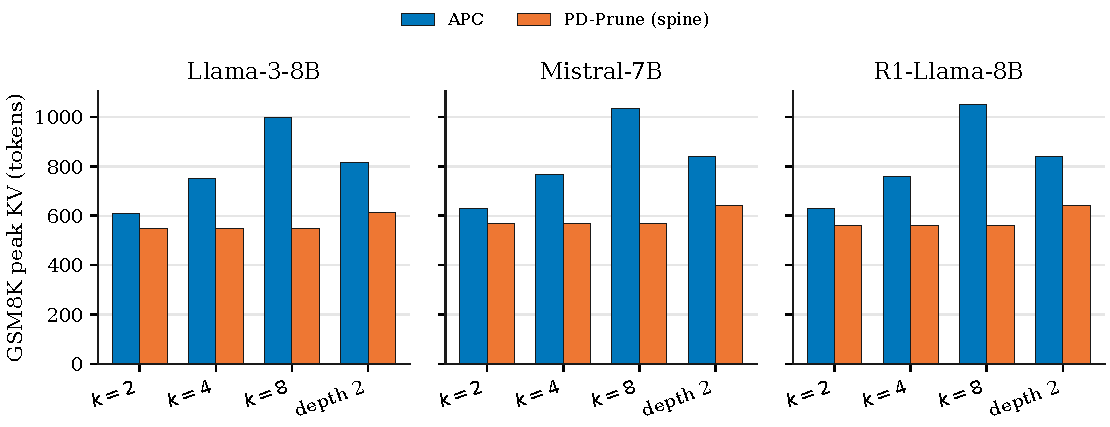
\includegraphics[width=\columnwidth]{fig/branch_peak.pdf}
\caption{\textbf{GSM8K peak KV versus branching} ($n{=}16$, $\mathrm{tp}{=}2$, $D{=}512$).
The spine peak (\sys and \cowonly) is invariant in $k$, while the APC peak grows with $k$.}
\label{fig:eval-branch}
\end{figure}

\Cref{tab:longcot} reports contest problems with $D{=}2048$ (MATH-500 $n{=}200$, AIME $n{=}73$).
The peak ratio is $0.78$--$0.91$, and accuracy is within $3$ points of APC on MATH-500 and within one problem on AIME.
We do not compare end-to-end time here: the APC harness decodes the full budget for every item, whereas ours stops at EOS, so time differences would reflect the harnesses rather than the methods.
The trunk token counts of the two harnesses also differ slightly (e.g., $95$ vs.\ $73$ on R1-8B MATH-500) because of prompt templating, which adds an offset to the ratios.

\begin{table}[t]
\centering
\caption{Contest problems, $D{=}2048$, $k{=}4$, $\mathrm{tp}{=}2$.
All rows of a model come from the same run.}
\label{tab:longcot}
\scriptsize
\setlength{\tabcolsep}{3.0pt}
\begin{tabular}{@{}llrrr@{}}
\toprule
Setting & System & peak & / APC & acc. \\
\midrule
 & APC & $1863$ & --- & $0.560$ \\
\rowcolor{tblalt}
 & \cowonly & \win{$1599$} & \win{$0.86$} & $0.530$ \\
\multirow{-3}{*}{R1-8B MATH} & \sys & \win{$1599$} & \win{$0.86$} & $0.530$ \\
\midrule
 & APC & $2118$ & --- & $0.041$ \\
\rowcolor{tblalt}
 & \cowonly & \win{$1662$} & \win{$0.78$} & $0.041$ \\
\multirow{-3}{*}{R1-8B AIME} & \sys & \win{$1662$} & \win{$0.78$} & $0.041$ \\
\midrule
 & APC & $1937$ & --- & $0.620$ \\
\rowcolor{tblalt}
 & \cowonly & \win{$1770$} & \win{$0.91$} & $0.625$ \\
\multirow{-3}{*}{Qwen3-4B MATH} & \sys & \win{$1770$} & \win{$0.91$} & $0.600$ \\
\midrule
 & APC & $2150$ & --- & $0.027$ \\
\rowcolor{tblalt}
 & \cowonly & \win{$1794$} & \win{$0.83$} & $0.041$ \\
\multirow{-3}{*}{Qwen3-4B AIME} & \sys & \win{$1794$} & \win{$0.83$} & $0.041$ \\
\bottomrule
\end{tabular}
\end{table}
